\section{Hierarchical non-linear dynamical system}\label{chapter-05:section:hierarchical-filter}

For our last example, we consider modeling a \ac{hnds}, 
which is a class of complex mathematical models used to describe and analyze the
behavior of dynamic processes with multiple levels of interactions and dependencies.
These systems involve interconnected components that can influence each other's dynamics, and, as in the previous example, exhibit nonlinear behaviors.
In an \ac{hnds}, the components are organized in a hierarchical structure, with higher-level
components influencing the behavior of lower-level components.
This hierarchical organization allows for the modeling of complex interactions and feedback
loops that are commonly found in real-world systems.

\subsection{Example of a hierarchical nonlinear dynamical system}

As a specific example of an \ac{hnds}, we consider the \acf{hgf}.
The \ac{hgf} model is well known in the computational neuroscience literature and is often used for
Bayesian modeling of volatile environments, such as uncertainty in perception
\citep{mathys_uncertainty_2014, iglesias_hierarchical_2013, paulus_roadmap_2016}.
Additionally, it finds applications in financial data analysis \citep{senoz_switching_2021}  (\hyperlink{experiments:utility}{\emph{Utility}}).
The \ac{hgf} can be described as a Gaussian random walk, where the time-varying variance of the
random walk is determined by the state of a higher-level process, for instance, a Gaussian
random walk with fixed volatility or another more complex signal.
Specifically, a simple \ac{hgf} model with $K$ layers can be defined as follows:
\begin{equation}
  \label{eq:sim:hgf}
  \begin{aligned}
    s^{(K)}_t & = s^{(K)}_{t - 1} +
    v^{(K)}_t,~~v^{(K)}_t \sim \mathcal{N}(0, \Sigma)                               \\ \cdots & \\ s^{(2)}_t & =
    s^{(2)}_{t - 1} + v^{(2)}_t,~~v^{(2)}_t \sim \mathcal{N}(0, f^{(2)}(s^{(2)}_t)) \\
    s^{(1)}_t & = s^{(1)}_{t - 1} + v^{(1)}_t,~~v^{(1)}_t \sim \mathcal{N}(0,
    f^{(1)}(s^{(2)}_t)                                                                        \\ y_t & = s^{(1)}_t + w_t,~~w_t \sim \mathcal{N}(0, \Omega)
  \end{aligned}
\end{equation} 
In these equations, $s^{(k)}_t$ represents the hidden state of the $k$-th layer of the
system at time $t$, $y_t$ is the observation at time $t$, and $f^{(k)}$ is a link function
that maps states from the $(k + 1)$-th layer to the nonnegative variance of the random walk in
the $k$-th layer.
Importantly, an \ac{hgf} model can have an arbitrary number of layers.
In terms of probability densities, the model can be expressed as 
\begin{equation}
  \label{eq:sim:hgf_probabilities}
  \begin{aligned}
    p(s^{(k)}_t \vert s^{(k)}_{t - 1}) & =
    \mathcal{N}(s^{(k)}_t \vert s^{(k)}_{t - 1}, \Sigma)                                  \\ \cdots & \\ p(s^{(2)}_t \vert
    s^{(2)}_{t - 1}, s^{(3)}_t)        & = \mathcal{N}(s^{(2)}_{t} \vert s^{(2)}_{t - 1},
    f^{(2)}(s^{(3)}_t))                                                                   \\ p(s^{(1)}_t \vert s^{(1)}_{t - 1}, s^{(2)}_t) & =
    \mathcal{N}(s^{(1)}_{t} \vert s^{(1)}_{t - 1}, f^{(1)}(s^{(2)}_t))                    \\ p(y_t \vert s^{(1)}_t) &
       = \mathcal{N}(y_t \vert s^{(1)}_t, \Omega)
  \end{aligned}
\end{equation} which is a hierarchical nonlinear state-space model.
The full probabilistic model can then be written as \begin{equation}
  \begin{aligned}
    \label{eq:sim:hgf_model} p(\bm{y}, \bm{s}, \Sigma, \Omega) =
    \underbrace{p(\Sigma)p(\Omega)\prod_{k = 1}^{K}p(s_1^{(k)})}_{\mathrm{prior}}\underbrace{\prod_{t = 1}^{T}p(y_t
      \vert s^{(1)}_t)}_{\mathrm{likelihood}} \underbrace{\prod_{t = 2}^{T}\prod_{k = 1}^{K}p(s^{(k)}_t \vert
      s^{(k)}_{t - 1}, s^{(k + 1)}_t)}_{\mathrm{state~transitions}}.
  \end{aligned}
\end{equation} The
Figure~\ref{fig:sim:hgf_model_graph} shows a \ac{tffg} representation of the
model~\eqref{eq:sim:hgf_model} with 2 layers of hierarchy with an arbitrary link function $f$.

\begin{figure}
  \centering
  \resizebox{\textwidth}{!}{\begin{tikzpicture}
  \node[] (splink) {$\cdots$};
  \node[box, node distance=3mm] (spN) [right=of splink] {$\mathcal{N}$};
  \node[smallbox] (speq) [right=of spN] {\small $=$};
  \node[box, node distance=5mm] (spfN) [right=of speq] {$\mathcal{N}$};
  \node[box, node distance=3mm] (spg) [below=of speq] {$f$};
  \node[box, node distance=3mm] (spgN) [below=of spg] {$\mathcal{N}$};

  \path[line] (splink) edge[-] (spN);
  \path[line] (spN) edge[-] node[pos=0.5, anchor=south]{$s^{(2)}_{t - 1}$} (speq);
  \path[line] (speq) edge[-] (spfN);
  \path[line] (speq) edge[-] (spg);
  \path[line] (spg) edge[-] node[pos=0.5, anchor=east](spgleft){} node[pos=0.5, anchor=west](spgright){} (spgN);

  \node[smallbox] (seq) [right=of spfN] {\small $=$};
  \node[box, node distance=5mm] (sfN) [right=of seq] {$\mathcal{N}$};
  \node[box, node distance=3mm] (sg) [below=of seq] {$f$};
  \node[box, node distance=3mm] (sgN) [below=of sg] {$\mathcal{N}$};

  \path[line] (spfN) edge[-] node[pos=0.5, anchor=south]{$s^{(2)}_{t}$} (seq);
  \path[line] (seq) edge[-] (sfN);
  \path[line] (seq) edge[-] (sg);
  \path[line] (sg) edge[-] node[pos=0.5, anchor=east](sgleft){} node[pos=0.5, anchor=west](sgright){} (sgN);

  \node[] (snlink) [right=of sfN] {$\cdots$};
  \node[box, node distance=5mm] (sTN) [right=of snlink] {$\mathcal{N}$};
  \node[smallbox, draw=white, node distance=5mm] (sTeq) [right=of sTN] {};
  \node[box, node distance=3mm] (sTg) [below=of sTeq] {$f$};
  \node[box, node distance=3mm] (sTgN) [below=of sTg] {$\mathcal{N}$};

  \path[line] (sfN) edge[-] node[pos=0.5, anchor=south]{$s^{(2)}_{t + 1}$} (snlink);
  \path[line] (snlink) edge[-] (sTN);
  \path[line] (sTN) edge[-] node[pos=0.5, anchor=south]{$s^{(2)}_T$} (sTeq.center);
  \draw[] (sTeq.center) -- (sTg);
  \path[line] (sTg) edge[-] node[pos=0.5, anchor=east](sTgleft){} node[pos=0.5, anchor=west](sTgright){} (sTgN);

  \node[box] (s0) [left=of splink] {$p(s^{(2)}_1)$};
  \path[line] (s0) edge[-] node[pos=0.5, anchor=south]{$s^{(2)}_1$} (splink);

  \node[smallbox] (pPsp) [above=of spN] {\small $=$};
  \node[node distance=4mm] (pPlink) [left=of pPsp] {$\cdots$};
  \node[box] (pP) [left=of pPlink] {$p(\Sigma)$};
  \node[smallbox] (pPs) [above=of spfN] {\small $=$};
  \node[smallbox] (pPsn) [above=of sfN] {\small $=$};
  \node[smallbox, draw=white] (pPsTeq) [right=of pPsn] {$\cdots$};

  \path[line] (pP) edge[-] node[pos=0.5, anchor=south]{$\Sigma$} (pPlink);
  \path[line] (pPlink) edge[-] (pPsp);
  \path[line] (pPsp) edge[-] (pPs);
  \path[line] (pPs) edge[-] (pPsn);
  \path[line] (pPsn) edge[-] (pPsTeq);
  \path[line] (pPsp) edge[-] (spN);
  \path[line] (pPs) edge[-] (spfN);
  \path[line] (pPsn) edge[-] (sfN);
  \draw[] (pPsTeq) -| (sTN);

  \node[smallbox, node distance=5mm] (lxpN) [left=of spgN] {\small $=$};
  \node[smallbox, node distance=5mm] (lxN) [left=of sgN] {\small $=$};
  \node[smallbox, node distance=5mm] (lxTN) [left=of sTgN] {\small $=$};
  \node[node distance=9mm] (lxplink) [left=of lxpN] {$\cdots$};
  \node[box] (px) [left=of lxplink] {$p(s^{(1)}_1)$};
  \node[] (lxlink1) [right=of sgN] {$\cdots$};
  \node[] (lxlink2) [left=of lxTN] {$\cdots$};

  \path[line] (px) edge[-] node[pos=0.5, anchor=south]{$s^{(1)}_1$} (lxplink);
  \path[line] (lxplink) edge[-] node[pos=0.5, anchor=south]{$s^{(1)}_{t - 2}$} (lxpN);
  \path[line] (lxpN) edge[-] (spgN);
  \path[line] (spgN) edge[-] node[pos=0.5, anchor=south]{$s^{(1)}_{t - 1}$} (lxN);
  \path[line] (lxN) edge[-] (sgN);
  \path[line] (sgN) edge[-] node[pos=0.5, anchor=south]{$s^{(1)}_{t}$} (lxlink1); 
  \path[line] (lxlink2) edge[-] node[pos=0.5, anchor=south]{$s^{(1)}_{T-1}$} (lxTN); 
  \path[line] (lxTN) edge[-] (sTgN);

  \node[box, node distance=13.5mm] (ypN) [below=of lxpN] {$\mathcal{N}$};
  \node[box, node distance=13.5mm] (yN) [below=of lxN] {$\mathcal{N}$};
  \node[box, node distance=13.5mm] (yTN) [below=of lxTN] {$\mathcal{N}$};
  \node[box, node distance=15mm] (yTTN) [right=of yTN] {$\mathcal{N}$};

  \path[line] (lxpN) edge[-] node[pos=0.5, anchor=east](xpleft){} node[pos=0.5, anchor=west](xpright){} (ypN);
  \path[line] (lxN) edge[-] node[pos=0.5, anchor=east](xleft){} node[pos=0.5, anchor=west](xright){} (yN);
  \path[line] (lxTN) edge[-] node[pos=0.5, anchor=east](xTleft){} node[pos=0.5, anchor=west](xTright){} (yTN);

  \node[smallbox, node distance=5mm] (nspeq) [left=of xpleft] {\small $=$};
  \node[smallbox, node distance=5mm] (nseq) [left=of xleft] {\small $=$};
  \node[smallbox, node distance=5mm] (nsTeq) [left=of xTleft] {\small $=$};
  \node[] (nlink1) [right=of xright] {$\cdots$};
  \node[] (nlink2) [left=of nsTeq] {$\cdots$};
  \node[] (nlink3) [right=of xTright] {};

  \draw[] (nspeq) -- (xpleft.center);
  \draw[] (xpright.center) -- (nseq);
  \draw[] (nseq) -- (xleft.center);
  \draw[] (xright.center) -- (nlink1);
  \draw[] (nlink2) -- (nsTeq);
  \draw[] (nsTeq) -- (xTleft.center);
  \draw[] (xTright.center) -- (nlink3.center);

  \draw[] (nspeq) |- (ypN);
  \draw[] (nseq) |- (yN);
  \draw[] (nsTeq) |- (yTN);
  \draw[] (nlink3.center) |- (yTTN);

  \node[node distance=3mm] (nlink0) [left=of nspeq] {$\cdots$};
  \node[box, node distance=8mm] (pomega) [left=of nlink0] {$p(\Omega)$};
  \path[line] (nlink0) edge[-] (nspeq);
  \path[line] (pomega) edge[-] node[pos=0.5, anchor=south]{$\Omega$} (nlink0);

  \node[clamped, node distance=5mm] (yp) [below=of ypN] {};
  \node[clamped, node distance=5mm] (y) [below=of yN] {};
  \node[clamped, node distance=5mm] (yT) [below=of yTN] {};
  \node[clamped, node distance=5mm] (yTT) [below=of yTTN] {};
  \path[line] (ypN) edge[-] node[pos=0.5, anchor=west]{$y_{t - 2}$} (yp);
  \path[line] (yN) edge[-] node[pos=0.5, anchor=west]{$y_{t - 1}$} (y);
  \path[line] (yTN) edge[-] node[pos=0.5, anchor=west]{$y_{T - 1}$} (yT);
  \path[line] (yTTN) edge[-] node[pos=0.5, anchor=west]{$y_{T}$} (yTT);

  \draw[] (sTgN) -| (yTTN);

\end{tikzpicture}

}
  \caption{An \ac{tffg} representation of the probabilistic model~\eqref{eq:sim:hgf_model} for a 2-layer \ac{hgf} system~\eqref{eq:sim:hgf}.
    $s^{(k)}_t$ together with $\Sigma$ and $\Omega$ are latent states, $y_t$ represents observations, and $f$ is an arbitrary link function.
    The symbol $\cdots$ denotes the repetitive structure of the corresponding graph.
  }
  \label{fig:sim:hgf_model_graph}
\end{figure}

\subsubsection*{Continual inference on infinite dataset}


In this example, our objective is to demonstrate online reactive Bayesian learning (filtering)
in a 2-layer \ac{hgf} model, as discussed in
Section~\ref{chapter-03:section:reactive-continual-inference}. More formally, we are interested in computing 
\begin{equation}
    \begin{split}
        p(s_t\vert \hat{\bm{y}}_{1:t}) &= \int p(\Sigma, \Omega, \bm{s}_{1:t}, \bm{y}_{1:t}) \prod_{i = 1}^{t}\delta(y_i - \hat{y}_i)\mathrm{d}\Sigma\mathrm{d}\Omega\mathrm{d}\Sigma\mathrm{d}\bm{s}_{1:t-1}\mathrm{d}\bm{y}_{1:t}
    \end{split}
\end{equation}
To achieve this in the \ac{rmp} framework, we only need to create a single time section of the corresponding graph instead of the full model graph, as has been discussed in Section~\ref{chapter-03:section:reactive-continual-inference}.
We will utilize the posterior information from time step index $t - 1$ as prior information for time
step index $t$.
It is worth noting that there are no inherent limitations to running this model on a full
graph, as has been shown in the previous examples.
In fact, \citep{mathys_hierarchical_2012} recommends using "batched" inference on the full
graph for the estimation of the parameters of the \ac{hgf} model to achieve better estimates.
However, "batch" parameter estimation may not be well-suited to track nonstationarities in real-time datasets, which are often present in real-world scenarios \citep{senoz_thesis, senoz_switching_2021}. 
The RxInfer framework is capable of performing the inference task in either case, allowing for
evaluation of the benefits of both approaches on a case-by-case basis.

\subsubsection*{Simulated measurements}

In the following experiments, we assume the use of the specific link function $f(s) =
  \exp(\kappa s + \zeta)$, which was previously mentioned in
Section~\ref{chapter-04:section:inference-customization}.
Figure~\ref{fig:rxi:gcv} illustrates a \ac{tffg} representation of this link function.
For simplicity and to avoid additional complexity in the model specification and its
corresponding \ac{tffg} representation, we fix the parameters $\kappa$ and $\zeta$.
However, it is important to note that there are no inherent limitations in making them random
variables, assigning priors to them, and estimating their posterior distributions.
Moreover, in the model defined by equation~\eqref{eq:sim:nlds}, we assume that the exact
distributions of the noise components $v_t$ and $w_t$ are unknown.
We also assume that the time difference (elapsed time) between two observations is fixed and known.
Figure~\ref{fig:sim:hgf_one_time_segment} shows a \ac{tffg} representation of the \ac{hgf} model~\eqref{eq:sim:hgf_model} in the filtering setting.
Additionally, Figures~\ref{fig:sim:hgf_example_states} illustrate the first $10,000$ time
steps of a simulated evolution along with the corresponding observations.

\begin{figure}
  \centering
  
\begin{tikzpicture}
  \node[smallbox] (mul) {$\times$};
  \node[smallbox, node distance=4mm] (plus) [below=of mul] {\small +};
  \node[smallbox, node distance=4mm] (exp) [below=of plus] {\small exp};
  \node[smallbox, node distance=4mm] (N) [below=of exp] {$\mathcal{N}$};

  \node[node distance=6mm] (z) [above=of mul] {};
  \node[box] (pz) [left=of z] {$\mathcal{N}$};
  \node[box, node distance=5mm] (ppz) [left=of pz] {$p(s^{(2)}_{t - 1})$};
  \node[] (zn) [right=of z] {};
  \node[clamped, node distance=6mm] (k) [left=of mul] {};
  \node[clamped, node distance=6mm] (w) [right=of plus] {};
  \node[box, node distance=12mm] (x) [left=of N] {$p(s^{(1)}_{t - 1})$};
  \node[node distance=12mm] (xn) [right=of N] {};
  \node[box, node distance=6mm] (yN) [below=of xn] {$\mathcal{N}$};
  \node[clamped, node distance=5mm] (y) [below=of yN] {}; 
  \node[box, node distance=5mm] (sigma) [above=of pz] {$p(\Sigma)$};
  \node[box, node distance=5mm] (omega) [left=of yN] {$p(\Omega)$};

  \draw[] (ppz) edge[-] (pz);
  \draw[] (pz) edge[-] node[pos=0.5, anchor=south]{$s^{(2)}_t$} (z.center);
  % \draw[] (z) edge[-] (zn);

  \draw[] (z.center) edge[-] node[pos=0.2, anchor=east]{} (mul);
  \draw[] (mul) edge[-] (plus);
  \draw[] (k) edge[-] node[pos=0.3, anchor=south]{$\kappa$} (mul);
  \draw[] (plus) edge[-] (exp);
  \draw[] (w) edge[-] node[pos=0.3, anchor=south]{$\zeta$} (plus);
  \draw[] (exp) edge[-] (N);
  \draw[] (x) edge[-] node[pos=0.5, anchor=south]{$s^{(1)}_{t - 1}$} (N);
  \draw[] (N) edge[-] node[pos=0.5, anchor=south]{$s^{(1)}_{t}$} (xn.center);
  \draw[] (xn.center) edge[-] (yN);
  \draw[] (yN) edge[-] node[pos=0.5, anchor=west]{$y_t$} (y);
  \draw[] (sigma) edge[-] (pz);
  \draw[] (omega) edge[-] (yN);

  \node[box, densely dotted, inner sep=2mm, label={[above right, xshift=5mm, yshift=-4mm]:{GCV}}] (bbox) [fit=(mul)(N)] {};
\end{tikzpicture}

  % \resizebox{\textwidth}{!}{
\begin{tikzpicture}
  \node[smallbox] (mul) {$\times$};
  \node[smallbox, node distance=4mm] (plus) [below=of mul] {\small +};
  \node[smallbox, node distance=4mm] (exp) [below=of plus] {\small exp};
  \node[smallbox, node distance=4mm] (N) [below=of exp] {$\mathcal{N}$};

  \node[node distance=6mm] (z) [above=of mul] {};
  \node[box] (pz) [left=of z] {$\mathcal{N}$};
  \node[box, node distance=5mm] (ppz) [left=of pz] {$p(s^{(2)}_{t - 1})$};
  \node[] (zn) [right=of z] {};
  \node[clamped, node distance=6mm] (k) [left=of mul] {};
  \node[clamped, node distance=6mm] (w) [right=of plus] {};
  \node[box, node distance=12mm] (x) [left=of N] {$p(s^{(1)}_{t - 1})$};
  \node[node distance=12mm] (xn) [right=of N] {};
  \node[box, node distance=6mm] (yN) [below=of xn] {$\mathcal{N}$};
  \node[clamped, node distance=5mm] (y) [below=of yN] {}; 
  \node[box, node distance=5mm] (sigma) [above=of pz] {$p(\Sigma)$};
  \node[box, node distance=5mm] (omega) [left=of yN] {$p(\Omega)$};

  \draw[] (ppz) edge[-] (pz);
  \draw[] (pz) edge[-] node[pos=0.5, anchor=south]{$s^{(2)}_t$} (z.center);
  % \draw[] (z) edge[-] (zn);

  \draw[] (z.center) edge[-] node[pos=0.2, anchor=east]{} (mul);
  \draw[] (mul) edge[-] (plus);
  \draw[] (k) edge[-] node[pos=0.3, anchor=south]{$\kappa$} (mul);
  \draw[] (plus) edge[-] (exp);
  \draw[] (w) edge[-] node[pos=0.3, anchor=south]{$\zeta$} (plus);
  \draw[] (exp) edge[-] (N);
  \draw[] (x) edge[-] node[pos=0.5, anchor=south]{$s^{(1)}_{t - 1}$} (N);
  \draw[] (N) edge[-] node[pos=0.5, anchor=south]{$s^{(1)}_{t}$} (xn.center);
  \draw[] (xn.center) edge[-] (yN);
  \draw[] (yN) edge[-] node[pos=0.5, anchor=west]{$y_t$} (y);
  \draw[] (sigma) edge[-] (pz);
  \draw[] (omega) edge[-] (yN);

  \node[box, densely dotted, inner sep=2mm, label={[above right, xshift=5mm, yshift=-4mm]:{GCV}}] (bbox) [fit=(mul)(N)] {};
\end{tikzpicture}
}
  \caption{A \ac{tffg} representation of a single time-segment of the probabilistic model~\eqref{eq:sim:hgf_model} for a 2-layer \ac{hgf} system~\eqref{eq:sim:hgf} with $f(s) =
      \exp(\kappa s + \zeta)$ as the link function.
    $s^{(k)}_t$ together with $\Sigma$ and $\Omega$ are latent states, $y_t$ are observations.
  }
  \label{fig:sim:hgf_one_time_segment}
\end{figure}

\begin{figure}
  \centering
  \begin{subfigure}[t]{0.475\textwidth}
    \centering
    \resizebox{\textwidth}{!}{
        % % Recommended preamble:
% \usetikzlibrary{arrows.meta}
% \usetikzlibrary{backgrounds}
% \usepgfplotslibrary{patchplots}
% \usepgfplotslibrary{fillbetween}
% \pgfplotsset{%
%     layers/standard/.define layer set={%
%         background,axis background,axis grid,axis ticks,axis lines,axis tick labels,pre main,main,axis descriptions,axis foreground%
%     }{
%         grid style={/pgfplots/on layer=axis grid},%
%         tick style={/pgfplots/on layer=axis ticks},%
%         axis line style={/pgfplots/on layer=axis lines},%
%         label style={/pgfplots/on layer=axis descriptions},%
%         legend style={/pgfplots/on layer=axis descriptions},%
%         title style={/pgfplots/on layer=axis descriptions},%
%         colorbar style={/pgfplots/on layer=axis descriptions},%
%         ticklabel style={/pgfplots/on layer=axis tick labels},%
%         axis background@ style={/pgfplots/on layer=axis background},%
%         3d box foreground style={/pgfplots/on layer=axis foreground},%
%     },
% }

\begin{tikzpicture}[/tikz/background rectangle/.style={fill={rgb,1:red,1.0;green,1.0;blue,1.0}, fill opacity={1.0}, draw opacity={1.0}}, show background rectangle]
\begin{axis}[point meta max={nan}, point meta min={nan}, legend cell align={left}, legend columns={1}, title={}, title style={at={{(0.5,1)}}, anchor={south}, font={{\fontsize{18 pt}{23.400000000000002 pt}\selectfont}}, color={rgb,1:red,0.0;green,0.0;blue,0.0}, draw opacity={1.0}, rotate={0.0}, align={center}}, legend style={color={rgb,1:red,0.0;green,0.0;blue,0.0}, draw opacity={1.0}, line width={1}, solid, fill={rgb,1:red,1.0;green,1.0;blue,1.0}, fill opacity={1.0}, text opacity={1.0}, font={{\fontsize{14 pt}{18.2 pt}\selectfont}}, text={rgb,1:red,0.0;green,0.0;blue,0.0}, cells={anchor={center}}, at={(0.02, 0.02)}, anchor={south west}}, axis background/.style={fill={rgb,1:red,1.0;green,1.0;blue,1.0}, opacity={1.0}}, anchor={north west}, xshift={1.0mm}, yshift={-1.0mm}, width={99.6mm}, height={74.2mm}, scaled x ticks={false}, xlabel={Time step index}, x tick style={color={rgb,1:red,0.0;green,0.0;blue,0.0}, opacity={1.0}}, x tick label style={color={rgb,1:red,0.0;green,0.0;blue,0.0}, opacity={1.0}, rotate={0}}, xlabel style={at={(ticklabel cs:0.5)}, anchor=near ticklabel, at={{(ticklabel cs:0.5)}}, anchor={near ticklabel}, font={{\fontsize{16 pt}{20.8 pt}\selectfont}}, color={rgb,1:red,0.0;green,0.0;blue,0.0}, draw opacity={1.0}, rotate={0.0}}, xmajorgrids={true}, xmin={-277.0}, xmax={10217.0}, xticklabels={{$0$,$2500$,$5000$,$7500$,$10000$}}, xtick={{0.0,2500.0,5000.0,7500.0,10000.0}}, xtick align={inside}, xticklabel style={font={{\fontsize{14 pt}{18.2 pt}\selectfont}}, color={rgb,1:red,0.0;green,0.0;blue,0.0}, draw opacity={1.0}, rotate={0.0}}, x grid style={color={rgb,1:red,0.0;green,0.0;blue,0.0}, draw opacity={0.1}, line width={0.5}, solid}, axis x line*={left}, x axis line style={color={rgb,1:red,0.0;green,0.0;blue,0.0}, draw opacity={1.0}, line width={1}, solid}, scaled y ticks={false}, ylabel={}, y tick style={color={rgb,1:red,0.0;green,0.0;blue,0.0}, opacity={1.0}}, y tick label style={color={rgb,1:red,0.0;green,0.0;blue,0.0}, opacity={1.0}, rotate={0}}, ylabel style={at={(ticklabel cs:0.5)}, anchor=near ticklabel, at={{(ticklabel cs:0.5)}}, anchor={near ticklabel}, font={{\fontsize{16 pt}{20.8 pt}\selectfont}}, color={rgb,1:red,0.0;green,0.0;blue,0.0}, draw opacity={1.0}, rotate={0.0}}, ymajorgrids={true}, ymin={-0.8142488657820772}, ymax={0.2584571736615031}, yticklabels={{$-0.75$,$-0.50$,$-0.25$,$0.00$,$0.25$}}, ytick={{-0.75,-0.5,-0.25,0.0,0.25}}, ytick align={inside}, yticklabel style={font={{\fontsize{14 pt}{18.2 pt}\selectfont}}, color={rgb,1:red,0.0;green,0.0;blue,0.0}, draw opacity={1.0}, rotate={0.0}}, y grid style={color={rgb,1:red,0.0;green,0.0;blue,0.0}, draw opacity={0.1}, line width={0.5}, solid}, axis y line*={left}, y axis line style={color={rgb,1:red,0.0;green,0.0;blue,0.0}, draw opacity={1.0}, line width={1}, solid}, colorbar={false}]
    \addplot[color={rgb,1:red,0.3059;green,0.4745;blue,0.6549}, name path={c59592b9-01b8-4118-b64a-cc5f17040077}, draw opacity={1.0}, line width={2}, solid]
        table[row sep={\\}]
        {
            \\
            20.0  -0.017714363408717806  \\
            120.0  -0.03031981561889148  \\
            220.0  -0.07800584656637763  \\
            320.0  -0.04519637569374746  \\
            420.0  -0.1895501683882646  \\
            520.0  -0.13913084966651065  \\
            620.0  -0.08436277750576925  \\
            720.0  -0.09797280644765398  \\
            820.0  -0.16273269716836208  \\
            920.0  -0.17093628238947195  \\
            1020.0  -0.040487855729603374  \\
            1120.0  -0.07146781786101417  \\
            1220.0  -0.08137131947457325  \\
            1320.0  -0.08331049795742647  \\
            1420.0  -0.027082052108420053  \\
            1520.0  -0.020970920788733  \\
            1620.0  -0.03252297100148165  \\
            1720.0  -0.086440896874568  \\
            1820.0  0.11213137879371679  \\
            1920.0  0.08815498954468355  \\
            2020.0  0.14345061360549682  \\
            2120.0  0.1738527859331274  \\
            2220.0  0.10879263777994755  \\
            2320.0  0.11578974595019646  \\
            2420.0  0.21189099806617784  \\
            2520.0  0.17471603913173184  \\
            2620.0  0.1940969962494026  \\
            2720.0  0.22809756877159054  \\
            2820.0  0.098922235335671  \\
            2920.0  -0.05678279872933818  \\
            3020.0  -0.24475581600360727  \\
            3120.0  -0.2208990189017549  \\
            3220.0  -0.3717816414372628  \\
            3320.0  -0.29437667409377277  \\
            3420.0  -0.2547804879820489  \\
            3520.0  -0.28768061676987144  \\
            3620.0  -0.34658664027291913  \\
            3720.0  -0.27476348762155245  \\
            3820.0  -0.4045932962998529  \\
            3920.0  -0.5740173883824468  \\
            4020.0  -0.6308775952582358  \\
            4120.0  -0.5908993033096395  \\
            4220.0  -0.37771297964588096  \\
            4320.0  -0.44430788734534865  \\
            4420.0  -0.4782393466750803  \\
            4520.0  -0.3455428357818275  \\
            4620.0  -0.40794146878337273  \\
            4720.0  -0.3702044711798191  \\
            4820.0  -0.4436461419290132  \\
            4920.0  -0.4165204606850431  \\
            5020.0  -0.5447681612031563  \\
            5120.0  -0.6114824088606563  \\
            5220.0  -0.659415522369523  \\
            5320.0  -0.6597703176064015  \\
            5420.0  -0.5445400917547797  \\
            5520.0  -0.5570346671260175  \\
            5620.0  -0.6500542929659792  \\
            5720.0  -0.7725905542524371  \\
            5820.0  -0.7411114853817794  \\
            5920.0  -0.7838892608921646  \\
            6020.0  -0.7505524729662401  \\
            6120.0  -0.5483448523563014  \\
            6220.0  -0.5749361962229627  \\
            6320.0  -0.5861312430977571  \\
            6420.0  -0.522411917093636  \\
            6520.0  -0.6088670719475303  \\
            6620.0  -0.536545727208839  \\
            6720.0  -0.45758892375242727  \\
            6820.0  -0.25089382283913253  \\
            6920.0  -0.3005925555325212  \\
            7020.0  -0.41158857861972004  \\
            7120.0  -0.4895960418461227  \\
            7220.0  -0.6171390716217825  \\
            7320.0  -0.4585750650805316  \\
            7420.0  -0.4067140042212498  \\
            7520.0  -0.3789104419364966  \\
            7620.0  -0.3803157427107729  \\
            7720.0  -0.4412833610534849  \\
            7820.0  -0.46073681965898683  \\
            7920.0  -0.4574115909860456  \\
            8020.0  -0.42286771458994826  \\
            8120.0  -0.45621762002053007  \\
            8220.0  -0.4040413533620254  \\
            8320.0  -0.3835930733413548  \\
            8420.0  -0.32131668900844806  \\
            8520.0  -0.30230029914527945  \\
            8620.0  -0.2258579882256835  \\
            8720.0  -0.29642084043101585  \\
            8820.0  -0.36362618213865744  \\
            8920.0  -0.41054919683347724  \\
            9020.0  -0.4665089007710655  \\
            9120.0  -0.47557076349016303  \\
            9220.0  -0.4773433112965115  \\
            9320.0  -0.4877681450542384  \\
            9420.0  -0.5946407299602552  \\
            9520.0  -0.3562315069345538  \\
            9620.0  -0.40078300804689077  \\
            9720.0  -0.2682871133517609  \\
            9820.0  -0.32543610543080337  \\
            9920.0  -0.4094592664079163  \\
        }
        ;
    \addlegendentry {$s^{(2)}$}
\end{axis}
\end{tikzpicture}

        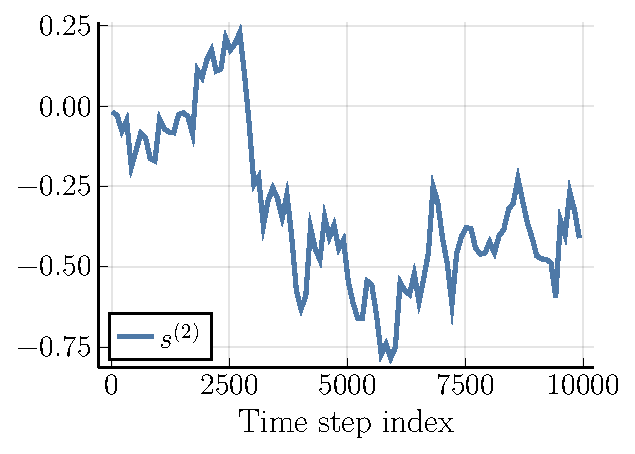
\includegraphics{contents/05-experiments/plots/hgf/04-hierarchical_example_states_1.pdf}
    }
    \caption{Simulated evolution of the layer $s_t^{(2)}$ at time-step index $t$.
    }
    \label{fig:sim:hgf_example_states_1}
  \end{subfigure}
  \hfill
  \begin{subfigure}[t]{0.475\textwidth}
    \centering
    \resizebox{\textwidth}{!}{
        % % Recommended preamble:
% \usetikzlibrary{arrows.meta}
% \usetikzlibrary{backgrounds}
% \usepgfplotslibrary{patchplots}
% \usepgfplotslibrary{fillbetween}
% \pgfplotsset{%
%     layers/standard/.define layer set={%
%         background,axis background,axis grid,axis ticks,axis lines,axis tick labels,pre main,main,axis descriptions,axis foreground%
%     }{
%         grid style={/pgfplots/on layer=axis grid},%
%         tick style={/pgfplots/on layer=axis ticks},%
%         axis line style={/pgfplots/on layer=axis lines},%
%         label style={/pgfplots/on layer=axis descriptions},%
%         legend style={/pgfplots/on layer=axis descriptions},%
%         title style={/pgfplots/on layer=axis descriptions},%
%         colorbar style={/pgfplots/on layer=axis descriptions},%
%         ticklabel style={/pgfplots/on layer=axis tick labels},%
%         axis background@ style={/pgfplots/on layer=axis background},%
%         3d box foreground style={/pgfplots/on layer=axis foreground},%
%     },
% }

\begin{tikzpicture}[/tikz/background rectangle/.style={fill={rgb,1:red,1.0;green,1.0;blue,1.0}, fill opacity={1.0}, draw opacity={1.0}}, show background rectangle]
\begin{axis}[point meta max={nan}, point meta min={nan}, legend cell align={left}, legend columns={1}, title={}, title style={at={{(0.5,1)}}, anchor={south}, font={{\fontsize{18 pt}{23.400000000000002 pt}\selectfont}}, color={rgb,1:red,0.0;green,0.0;blue,0.0}, draw opacity={1.0}, rotate={0.0}, align={center}}, legend style={color={rgb,1:red,0.0;green,0.0;blue,0.0}, draw opacity={1.0}, line width={1}, solid, fill={rgb,1:red,1.0;green,1.0;blue,1.0}, fill opacity={1.0}, text opacity={1.0}, font={{\fontsize{14 pt}{18.2 pt}\selectfont}}, text={rgb,1:red,0.0;green,0.0;blue,0.0}, cells={anchor={center}}, at={(0.98, 0.02)}, anchor={south east}}, axis background/.style={fill={rgb,1:red,1.0;green,1.0;blue,1.0}, opacity={1.0}}, anchor={north west}, xshift={1.0mm}, yshift={-1.0mm}, width={99.6mm}, height={74.2mm}, scaled x ticks={false}, xlabel={Time step index}, x tick style={color={rgb,1:red,0.0;green,0.0;blue,0.0}, opacity={1.0}}, x tick label style={color={rgb,1:red,0.0;green,0.0;blue,0.0}, opacity={1.0}, rotate={0}}, xlabel style={at={(ticklabel cs:0.5)}, anchor=near ticklabel, at={{(ticklabel cs:0.5)}}, anchor={near ticklabel}, font={{\fontsize{16 pt}{20.8 pt}\selectfont}}, color={rgb,1:red,0.0;green,0.0;blue,0.0}, draw opacity={1.0}, rotate={0.0}}, xmajorgrids={true}, xmin={-277.0}, xmax={10217.0}, xticklabels={{$0$,$2500$,$5000$,$7500$,$10000$}}, xtick={{0.0,2500.0,5000.0,7500.0,10000.0}}, xtick align={inside}, xticklabel style={font={{\fontsize{14 pt}{18.2 pt}\selectfont}}, color={rgb,1:red,0.0;green,0.0;blue,0.0}, draw opacity={1.0}, rotate={0.0}}, x grid style={color={rgb,1:red,0.0;green,0.0;blue,0.0}, draw opacity={0.1}, line width={0.5}, solid}, axis x line*={left}, x axis line style={color={rgb,1:red,0.0;green,0.0;blue,0.0}, draw opacity={1.0}, line width={1}, solid}, scaled y ticks={false}, ylabel={}, y tick style={color={rgb,1:red,0.0;green,0.0;blue,0.0}, opacity={1.0}}, y tick label style={color={rgb,1:red,0.0;green,0.0;blue,0.0}, opacity={1.0}, rotate={0}}, ylabel style={at={(ticklabel cs:0.5)}, anchor=near ticklabel, at={{(ticklabel cs:0.5)}}, anchor={near ticklabel}, font={{\fontsize{16 pt}{20.8 pt}\selectfont}}, color={rgb,1:red,0.0;green,0.0;blue,0.0}, draw opacity={1.0}, rotate={0.0}}, ymajorgrids={true}, ymin={-141.9838333878513}, ymax={-1.772464452523593}, yticklabels={{$-125$,$-100$,$-75$,$-50$,$-25$}}, ytick={{-125.0,-100.0,-75.0,-50.0,-25.0}}, ytick align={inside}, yticklabel style={font={{\fontsize{14 pt}{18.2 pt}\selectfont}}, color={rgb,1:red,0.0;green,0.0;blue,0.0}, draw opacity={1.0}, rotate={0.0}}, y grid style={color={rgb,1:red,0.0;green,0.0;blue,0.0}, draw opacity={0.1}, line width={0.5}, solid}, axis y line*={left}, y axis line style={color={rgb,1:red,0.0;green,0.0;blue,0.0}, draw opacity={1.0}, line width={1}, solid}, colorbar={false}]
    \addplot[color={rgb,1:red,0.6902;green,0.4784;blue,0.6314}, name path={1cd19579-c0eb-458b-8ca5-fd6c748a315c}, draw opacity={1.0}, line width={2}, solid]
        table[row sep={\\}]
        {
            \\
            20.0  -5.740710743146092  \\
            120.0  -16.612356409740595  \\
            220.0  -30.214939728674338  \\
            320.0  -27.91277108347563  \\
            420.0  -38.44051445158849  \\
            520.0  -36.37692770870293  \\
            620.0  -28.657499818104238  \\
            720.0  -38.11518859043452  \\
            820.0  -32.23811428629152  \\
            920.0  -28.365027552107573  \\
            1020.0  -30.315432575532842  \\
            1120.0  -46.81987978670828  \\
            1220.0  -46.48164775220454  \\
            1320.0  -33.32503463176701  \\
            1420.0  -35.15999677518617  \\
            1520.0  -35.71038384923469  \\
            1620.0  -40.893894030255126  \\
            1720.0  -39.25486028847835  \\
            1820.0  -50.349916409688475  \\
            1920.0  -51.076761742174455  \\
            2020.0  -58.43102646839949  \\
            2120.0  -69.68685913597517  \\
            2220.0  -63.75342245661089  \\
            2320.0  -73.28334225380378  \\
            2420.0  -76.26316055388325  \\
            2520.0  -115.40808732749156  \\
            2620.0  -110.50279837754361  \\
            2720.0  -95.30321841859855  \\
            2820.0  -92.8887102970675  \\
            2920.0  -110.80200605436752  \\
            3020.0  -119.46090050450783  \\
            3120.0  -126.5299510861929  \\
            3220.0  -121.32351826893401  \\
            3320.0  -125.60844688335281  \\
            3420.0  -133.01014303493668  \\
            3520.0  -138.0155870972288  \\
            3620.0  -129.5261427971083  \\
            3720.0  -122.27921209431543  \\
            3820.0  -120.3164502827986  \\
            3920.0  -113.13666947422665  \\
            4020.0  -113.97850179859742  \\
            4120.0  -125.88220598136336  \\
            4220.0  -126.85244318876003  \\
            4320.0  -118.38418716296158  \\
            4420.0  -111.73366972541768  \\
            4520.0  -119.88683501175005  \\
            4620.0  -92.83742376705094  \\
            4720.0  -91.08626110445321  \\
            4820.0  -86.11334335878445  \\
            4920.0  -78.78128167867484  \\
            5020.0  -77.71717298900397  \\
            5120.0  -76.64967150209743  \\
            5220.0  -72.17253805490954  \\
            5320.0  -80.28208366932938  \\
            5420.0  -72.2365997940903  \\
            5520.0  -54.560365734612056  \\
            5620.0  -57.51253985758529  \\
            5720.0  -70.10017754179482  \\
            5820.0  -68.86698992583172  \\
            5920.0  -78.63023427471254  \\
            6020.0  -84.03854154243193  \\
            6120.0  -79.84480016713425  \\
            6220.0  -79.68251647287082  \\
            6320.0  -88.5079577831925  \\
            6420.0  -93.20288652652177  \\
            6520.0  -85.8003987308885  \\
            6620.0  -80.24422203190426  \\
            6720.0  -76.24930449180981  \\
            6820.0  -64.60282044971704  \\
            6920.0  -64.09617045180755  \\
            7020.0  -68.902151721553  \\
            7120.0  -69.71453784822451  \\
            7220.0  -63.13519862587223  \\
            7320.0  -60.59210851070374  \\
            7420.0  -42.58328751848333  \\
            7520.0  -53.37883529178319  \\
            7620.0  -45.92453440684575  \\
            7720.0  -52.27878794361281  \\
            7820.0  -56.48992201341925  \\
            7920.0  -62.36671362460824  \\
            8020.0  -45.85998106666752  \\
            8120.0  -65.64823797939657  \\
            8220.0  -57.2476583848691  \\
            8320.0  -56.1917153444642  \\
            8420.0  -69.25777132654598  \\
            8520.0  -69.57230538642035  \\
            8620.0  -63.777346085996626  \\
            8720.0  -55.00392627071413  \\
            8820.0  -43.07094713280625  \\
            8920.0  -35.67458728809847  \\
            9020.0  -29.87085725414616  \\
            9120.0  -32.3540078567988  \\
            9220.0  -38.70973810006492  \\
            9320.0  -46.89969966114424  \\
            9420.0  -66.87691878358183  \\
            9520.0  -75.91034514738557  \\
            9620.0  -80.63209074519688  \\
            9720.0  -64.05168590602386  \\
            9820.0  -57.123291475702935  \\
            9920.0  -61.257290866591774  \\
        }
        ;
    \addlegendentry {$s^{(1)}$}
    \addplot[color={rgb,1:red,0.349;green,0.6314;blue,0.3098}, name path={e5a24211-ae00-4d62-9584-c87e53e39175}, only marks, draw opacity={0.5}, line width={0}, solid, mark={*}, mark size={1.5 pt}, mark repeat={1}, mark options={color={rgb,1:red,0.0;green,0.0;blue,0.0}, draw opacity={0.5}, fill={rgb,1:red,0.349;green,0.6314;blue,0.3098}, fill opacity={0.5}, line width={0.0}, rotate={0}, solid}]
        table[row sep={\\}]
        {
            \\
            20.0  -5.742770854791965  \\
            120.0  -17.2895289665243  \\
            220.0  -30.361340286844754  \\
            320.0  -27.704016346290324  \\
            420.0  -38.302895249889275  \\
            520.0  -36.677634111622766  \\
            620.0  -28.644058786972053  \\
            720.0  -38.141224988304835  \\
            820.0  -32.580190010420054  \\
            920.0  -28.63268053136293  \\
            1020.0  -30.721186493666398  \\
            1120.0  -46.40489702462974  \\
            1220.0  -46.99337372808301  \\
            1320.0  -33.05856626021657  \\
            1420.0  -35.452662992160825  \\
            1520.0  -36.21238580493504  \\
            1620.0  -41.31875559694605  \\
            1720.0  -39.078578990395606  \\
            1820.0  -50.63439290330427  \\
            1920.0  -51.086983322520624  \\
            2020.0  -58.361111038157105  \\
            2120.0  -70.00720496159775  \\
            2220.0  -63.690482907628954  \\
            2320.0  -73.79779244027957  \\
            2420.0  -76.34354013802468  \\
            2520.0  -115.61342839739346  \\
            2620.0  -110.41669342141986  \\
            2720.0  -95.34989752090296  \\
            2820.0  -93.12028579372817  \\
            2920.0  -110.66583791070892  \\
            3020.0  -119.5096387013258  \\
            3120.0  -126.30117533529366  \\
            3220.0  -121.18310402678331  \\
            3320.0  -125.40914331079675  \\
            3420.0  -133.06326899710115  \\
            3520.0  -137.96946127226911  \\
            3620.0  -129.44258604526055  \\
            3720.0  -121.71322100365353  \\
            3820.0  -120.71921825157227  \\
            3920.0  -113.22379873129485  \\
            4020.0  -113.62188174125336  \\
            4120.0  -126.46820918013178  \\
            4220.0  -126.93585357927385  \\
            4320.0  -118.35283789490236  \\
            4420.0  -111.29335819176698  \\
            4520.0  -119.90163627876177  \\
            4620.0  -92.43253286840418  \\
            4720.0  -91.07210968551689  \\
            4820.0  -85.68851702146705  \\
            4920.0  -79.15102338448396  \\
            5020.0  -77.88424675719315  \\
            5120.0  -76.59743529190374  \\
            5220.0  -71.90848144492746  \\
            5320.0  -80.73391791260532  \\
            5420.0  -71.95886687283739  \\
            5520.0  -54.5832402306863  \\
            5620.0  -57.31268120942707  \\
            5720.0  -70.15880529961798  \\
            5820.0  -68.9112088642401  \\
            5920.0  -78.71551797595836  \\
            6020.0  -84.35387311303546  \\
            6120.0  -79.81893822708403  \\
            6220.0  -78.94632055008643  \\
            6320.0  -88.45872943103531  \\
            6420.0  -93.03864950480617  \\
            6520.0  -85.69920440386407  \\
            6620.0  -80.17649312342434  \\
            6720.0  -76.37011098376705  \\
            6820.0  -64.7659676967172  \\
            6920.0  -64.25657293334554  \\
            7020.0  -68.79682725587386  \\
            7120.0  -69.47587744497314  \\
            7220.0  -63.04387302173695  \\
            7320.0  -60.89407673695217  \\
            7420.0  -42.55153056554662  \\
            7520.0  -53.63647523858669  \\
            7620.0  -46.130856025096804  \\
            7720.0  -52.67119451869334  \\
            7820.0  -56.92936871748146  \\
            7920.0  -62.58934108392828  \\
            8020.0  -45.71437237839573  \\
            8120.0  -65.68806834595546  \\
            8220.0  -57.24014878403126  \\
            8320.0  -56.018298242955666  \\
            8420.0  -69.38202679895872  \\
            8520.0  -69.66311027098386  \\
            8620.0  -63.57080652991492  \\
            8720.0  -54.875127370085764  \\
            8820.0  -42.95452380221737  \\
            8920.0  -35.910045616945354  \\
            9020.0  -29.40618005008118  \\
            9120.0  -32.42537960864664  \\
            9220.0  -38.7585851696836  \\
            9320.0  -47.067333417680416  \\
            9420.0  -66.78553207005805  \\
            9520.0  -76.07856038466359  \\
            9620.0  -80.69759584687029  \\
            9720.0  -63.87501906109672  \\
            9820.0  -57.12550346293002  \\
            9920.0  -61.13180115333624  \\
        }
        ;
    \addlegendentry {$y$}
\end{axis}
\end{tikzpicture}

        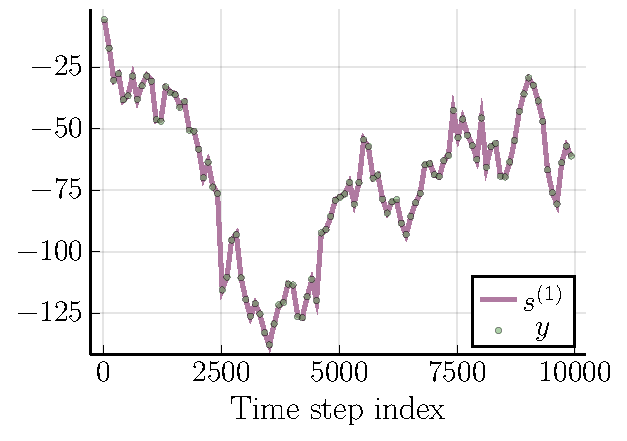
\includegraphics{contents/05-experiments/plots/hgf/04-hierarchical_example_states_2.pdf}
    }
    \caption{Simulated evolution of the layer $s_t^{(1)}$ and measurements $y$ at time-step index $t$.}
    \label{fig:sim:hgf_example_states_2}
  \end{subfigure}
  \caption{
    Simulated evolution of the 2-layer \ac{hgf} model \eqref{eq:sim:hgf_model} for $10,000$ synthetically generated 1-dimensional observations with link function $f(s) = exp(\kappa s + \zeta)$, where $\kappa = 1$ and $\zeta = 0$.
    The noise component $\Sigma$ is set to be $10^{-4}$, the noise component $\Omega$ is set to be
    $0.0625$.
  }
  \label{fig:sim:hgf_example_states}
\end{figure}

\subsection{The probabilistic model and the inference specification}
\begin{figure*}
  \begin{adjustbox}{minipage=\textwidth,margin=0pt \smallskipamount,center}
    \jlinputlisting[label={lst:sim:hgf_model_specification}, caption={An example of specification of the probabilistic 2-layer \ac{hgf} model~\eqref{eq:sim:hgf_model}.
        },captionpos=b]{contents/05-experiments/code/04-hgf-model.jl}
  \end{adjustbox}
\end{figure*}
Listing~\ref{lst:sim:hgf_model_specification} presents an example of the specification of the probabilistic 2-layer \ac{hgf} model~\eqref{eq:sim:hgf_model} using the RxInfer framework.
As part of the inference specification, we define extra factorization constraints for the
variational family of distributions $Q_{B}$ with the \jlinl{@constraints} macro.
The extra constraints assume that states $\bm{z}$, $\bm{x}$, and the precision of the
measurement noise are jointly independent.
\begin{figure*}
  \begin{adjustbox}{minipage=\textwidth,margin=0pt \smallskipamount,center}
    \jlinputlisting[label={lst:sim:hgf_constraints}, caption={Extra factorization constraints for the variational family of distributions $Q_{B}$ for the probabilistic model of the 2-layer \ac{hgf} system defined in Listing~\eqref{lst:sim:hgf_model_specification}.
        },captionpos=b]{contents/05-experiments/code/04-hgf-constraints.jl}
  \end{adjustbox}
\end{figure*}
In order to execute the inference procedure, we use the \jlinl{rxinference()} function, which
supports streaming datasets and continual inference.
The \jlinl{rxinference()} function subscribes to a data source and performs continual
inference as soon as new measurements become available.
In between measurements, while idle, the inference engine can perform additional \ac{vmp} iterations to
increase the accuracy of the estimated posteriors.
We use the \jlinl{@autoupdates} macro to specify how to update the prior information at time
step index $t$ using the posterior information from time step index $t - 1$.
Figure~\ref{fig:sim:hgf_inference_states} shows an example of the inference task and inferred
posterior distributions over states with their corresponding uncertainties.
For this type of model, the full model and inference specifications require around 40 lines of
code  (\hyperlink{experiments:userfriendliness}{\emph{User-friendliness}}).
\begin{figure*}
  \begin{adjustbox}{minipage=\textwidth,margin=0pt \smallskipamount,center}
    \jlinputlisting[label={lst:sim:hgf_inference}, caption={An example of the inference execution for the probabilistic model of the 2-layer \ac{hgf} model defined in Listing~\eqref{lst:sim:hgf_model_specification} with constraints defined in Listing~\ref{lst:sim:hgf_constraints}.
          The \jlinl{@autoupdates} macro specifies how to update the prior information at time step index $t$
          by using the posterior information from time step index $t - 1$.
        },captionpos=b]{contents/05-experiments/code/04-hgf-inference.jl}
  \end{adjustbox}
\end{figure*}

\begin{figure}
  \centering
  \begin{subfigure}[t]{0.315\textwidth}
    \centering
    \resizebox{\textwidth}{!}{
        % % Recommended preamble:
% \usetikzlibrary{arrows.meta}
% \usetikzlibrary{backgrounds}
% \usepgfplotslibrary{patchplots}
% \usepgfplotslibrary{fillbetween}
% \pgfplotsset{%
%     layers/standard/.define layer set={%
%         background,axis background,axis grid,axis ticks,axis lines,axis tick labels,pre main,main,axis descriptions,axis foreground%
%     }{
%         grid style={/pgfplots/on layer=axis grid},%
%         tick style={/pgfplots/on layer=axis ticks},%
%         axis line style={/pgfplots/on layer=axis lines},%
%         label style={/pgfplots/on layer=axis descriptions},%
%         legend style={/pgfplots/on layer=axis descriptions},%
%         title style={/pgfplots/on layer=axis descriptions},%
%         colorbar style={/pgfplots/on layer=axis descriptions},%
%         ticklabel style={/pgfplots/on layer=axis tick labels},%
%         axis background@ style={/pgfplots/on layer=axis background},%
%         3d box foreground style={/pgfplots/on layer=axis foreground},%
%     },
% }

\begin{tikzpicture}[/tikz/background rectangle/.style={fill={rgb,1:red,1.0;green,1.0;blue,1.0}, fill opacity={1.0}, draw opacity={1.0}}, show background rectangle]
\begin{axis}[point meta max={nan}, point meta min={nan}, legend cell align={left}, legend columns={1}, title={}, title style={at={{(0.5,1)}}, anchor={south}, font={{\fontsize{18 pt}{23.400000000000002 pt}\selectfont}}, color={rgb,1:red,0.0;green,0.0;blue,0.0}, draw opacity={1.0}, rotate={0.0}, align={center}}, legend style={color={rgb,1:red,0.0;green,0.0;blue,0.0}, draw opacity={1.0}, line width={1}, solid, fill={rgb,1:red,1.0;green,1.0;blue,1.0}, fill opacity={1.0}, text opacity={1.0}, font={{\fontsize{14 pt}{18.2 pt}\selectfont}}, text={rgb,1:red,0.0;green,0.0;blue,0.0}, cells={anchor={center}}, at={(0.02, 0.02)}, anchor={south west}}, axis background/.style={fill={rgb,1:red,1.0;green,1.0;blue,1.0}, opacity={1.0}}, anchor={north west}, xshift={1.0mm}, yshift={-1.0mm}, width={99.6mm}, height={74.2mm}, scaled x ticks={false}, xlabel={Time step index}, x tick style={color={rgb,1:red,0.0;green,0.0;blue,0.0}, opacity={1.0}}, x tick label style={color={rgb,1:red,0.0;green,0.0;blue,0.0}, opacity={1.0}, rotate={0}}, xlabel style={at={(ticklabel cs:0.5)}, anchor=near ticklabel, at={{(ticklabel cs:0.5)}}, anchor={near ticklabel}, font={{\fontsize{16 pt}{20.8 pt}\selectfont}}, color={rgb,1:red,0.0;green,0.0;blue,0.0}, draw opacity={1.0}, rotate={0.0}}, xmajorgrids={true}, xmin={-277.0}, xmax={10217.0}, xticklabels={{$0$,$2500$,$5000$,$7500$,$10000$}}, xtick={{0.0,2500.0,5000.0,7500.0,10000.0}}, xtick align={inside}, xticklabel style={font={{\fontsize{14 pt}{18.2 pt}\selectfont}}, color={rgb,1:red,0.0;green,0.0;blue,0.0}, draw opacity={1.0}, rotate={0.0}}, x grid style={color={rgb,1:red,0.0;green,0.0;blue,0.0}, draw opacity={0.1}, line width={0.5}, solid}, axis x line*={left}, x axis line style={color={rgb,1:red,0.0;green,0.0;blue,0.0}, draw opacity={1.0}, line width={1}, solid}, scaled y ticks={false}, ylabel={}, y tick style={color={rgb,1:red,0.0;green,0.0;blue,0.0}, opacity={1.0}}, y tick label style={color={rgb,1:red,0.0;green,0.0;blue,0.0}, opacity={1.0}, rotate={0}}, ylabel style={at={(ticklabel cs:0.5)}, anchor=near ticklabel, at={{(ticklabel cs:0.5)}}, anchor={near ticklabel}, font={{\fontsize{16 pt}{20.8 pt}\selectfont}}, color={rgb,1:red,0.0;green,0.0;blue,0.0}, draw opacity={1.0}, rotate={0.0}}, ymajorgrids={true}, ymin={-1.3490315915537232}, ymax={0.9652708372225225}, yticklabels={{$-1.0$,$-0.5$,$0.0$,$0.5$}}, ytick={{-1.0,-0.5,0.0,0.5}}, ytick align={inside}, yticklabel style={font={{\fontsize{14 pt}{18.2 pt}\selectfont}}, color={rgb,1:red,0.0;green,0.0;blue,0.0}, draw opacity={1.0}, rotate={0.0}}, y grid style={color={rgb,1:red,0.0;green,0.0;blue,0.0}, draw opacity={0.1}, line width={0.5}, solid}, axis y line*={left}, y axis line style={color={rgb,1:red,0.0;green,0.0;blue,0.0}, draw opacity={1.0}, line width={1}, solid}, colorbar={false}]
    \addplot[color={rgb,1:red,0.3059;green,0.4745;blue,0.6549}, name path={d51c1e62-caba-4845-b716-1b868951d96a}, draw opacity={1.0}, line width={2}, solid]
        table[row sep={\\}]
        {
            \\
            20.0  -0.017714363408717806  \\
            120.0  -0.03031981561889148  \\
            220.0  -0.07800584656637763  \\
            320.0  -0.04519637569374746  \\
            420.0  -0.1895501683882646  \\
            520.0  -0.13913084966651065  \\
            620.0  -0.08436277750576925  \\
            720.0  -0.09797280644765398  \\
            820.0  -0.16273269716836208  \\
            920.0  -0.17093628238947195  \\
            1020.0  -0.040487855729603374  \\
            1120.0  -0.07146781786101417  \\
            1220.0  -0.08137131947457325  \\
            1320.0  -0.08331049795742647  \\
            1420.0  -0.027082052108420053  \\
            1520.0  -0.020970920788733  \\
            1620.0  -0.03252297100148165  \\
            1720.0  -0.086440896874568  \\
            1820.0  0.11213137879371679  \\
            1920.0  0.08815498954468355  \\
            2020.0  0.14345061360549682  \\
            2120.0  0.1738527859331274  \\
            2220.0  0.10879263777994755  \\
            2320.0  0.11578974595019646  \\
            2420.0  0.21189099806617784  \\
            2520.0  0.17471603913173184  \\
            2620.0  0.1940969962494026  \\
            2720.0  0.22809756877159054  \\
            2820.0  0.098922235335671  \\
            2920.0  -0.05678279872933818  \\
            3020.0  -0.24475581600360727  \\
            3120.0  -0.2208990189017549  \\
            3220.0  -0.3717816414372628  \\
            3320.0  -0.29437667409377277  \\
            3420.0  -0.2547804879820489  \\
            3520.0  -0.28768061676987144  \\
            3620.0  -0.34658664027291913  \\
            3720.0  -0.27476348762155245  \\
            3820.0  -0.4045932962998529  \\
            3920.0  -0.5740173883824468  \\
            4020.0  -0.6308775952582358  \\
            4120.0  -0.5908993033096395  \\
            4220.0  -0.37771297964588096  \\
            4320.0  -0.44430788734534865  \\
            4420.0  -0.4782393466750803  \\
            4520.0  -0.3455428357818275  \\
            4620.0  -0.40794146878337273  \\
            4720.0  -0.3702044711798191  \\
            4820.0  -0.4436461419290132  \\
            4920.0  -0.4165204606850431  \\
            5020.0  -0.5447681612031563  \\
            5120.0  -0.6114824088606563  \\
            5220.0  -0.659415522369523  \\
            5320.0  -0.6597703176064015  \\
            5420.0  -0.5445400917547797  \\
            5520.0  -0.5570346671260175  \\
            5620.0  -0.6500542929659792  \\
            5720.0  -0.7725905542524371  \\
            5820.0  -0.7411114853817794  \\
            5920.0  -0.7838892608921646  \\
            6020.0  -0.7505524729662401  \\
            6120.0  -0.5483448523563014  \\
            6220.0  -0.5749361962229627  \\
            6320.0  -0.5861312430977571  \\
            6420.0  -0.522411917093636  \\
            6520.0  -0.6088670719475303  \\
            6620.0  -0.536545727208839  \\
            6720.0  -0.45758892375242727  \\
            6820.0  -0.25089382283913253  \\
            6920.0  -0.3005925555325212  \\
            7020.0  -0.41158857861972004  \\
            7120.0  -0.4895960418461227  \\
            7220.0  -0.6171390716217825  \\
            7320.0  -0.4585750650805316  \\
            7420.0  -0.4067140042212498  \\
            7520.0  -0.3789104419364966  \\
            7620.0  -0.3803157427107729  \\
            7720.0  -0.4412833610534849  \\
            7820.0  -0.46073681965898683  \\
            7920.0  -0.4574115909860456  \\
            8020.0  -0.42286771458994826  \\
            8120.0  -0.45621762002053007  \\
            8220.0  -0.4040413533620254  \\
            8320.0  -0.3835930733413548  \\
            8420.0  -0.32131668900844806  \\
            8520.0  -0.30230029914527945  \\
            8620.0  -0.2258579882256835  \\
            8720.0  -0.29642084043101585  \\
            8820.0  -0.36362618213865744  \\
            8920.0  -0.41054919683347724  \\
            9020.0  -0.4665089007710655  \\
            9120.0  -0.47557076349016303  \\
            9220.0  -0.4773433112965115  \\
            9320.0  -0.4877681450542384  \\
            9420.0  -0.5946407299602552  \\
            9520.0  -0.3562315069345538  \\
            9620.0  -0.40078300804689077  \\
            9720.0  -0.2682871133517609  \\
            9820.0  -0.32543610543080337  \\
            9920.0  -0.4094592664079163  \\
        }
        ;
    \addlegendentry {$z$}
    \addplot+[line width={0}, draw opacity={0}, fill={rgb,1:red,0.949;green,0.5569;blue,0.1686}, fill opacity={0.5}, mark={none}, forget plot]
        coordinates {
            (20,-0.13662375932419052)
            (120,-0.08886163728899887)
            (220,-0.14532020372812837)
            (320,-0.1298301037676746)
            (420,-0.16073027810209967)
            (520,-0.22531707024971168)
            (620,-0.22463414646110305)
            (720,-0.16055510594810044)
            (820,-0.2082474142725524)
            (920,-0.09801239289530621)
            (1020,-0.1548343174645875)
            (1120,-0.1536825667772715)
            (1220,-0.15504666702264916)
            (1320,-0.253556007033205)
            (1420,-0.21654166214854667)
            (1520,-0.18474593316153468)
            (1620,-0.14357873694384196)
            (1720,-0.2245407895447362)
            (1820,-0.10482461639257336)
            (1920,-0.1047704235413623)
            (2020,0.04976050317033892)
            (2120,0.2515122346886318)
            (2220,0.24567170175880207)
            (2320,0.23733979781810458)
            (2420,0.27905915254611335)
            (2520,0.3261128878563081)
            (2620,0.27619739660074205)
            (2720,0.1473221850819774)
            (2820,0.13658033913580653)
            (2920,0.033642292746779524)
            (3020,0.0015441871197079899)
            (3120,-0.041095223801829596)
            (3220,-0.13107923379443104)
            (3320,-0.31664686628296423)
            (3420,-0.26664194097315574)
            (3520,-0.27881112354389187)
            (3620,-0.22102855323490248)
            (3720,-0.21538657546444398)
            (3820,-0.3088094126125226)
            (3920,-0.39636412176160507)
            (4020,-0.5666901894831511)
            (4120,-0.6607849619168624)
            (4220,-0.6419621489555639)
            (4320,-0.6787529488492452)
            (4420,-0.6666055579824426)
            (4520,-0.5900007009787386)
            (4620,-0.4084347981814856)
            (4720,-0.4542304854948032)
            (4820,-0.49506352030839496)
            (4920,-0.5049067535967147)
            (5020,-0.5674875597343266)
            (5120,-0.5047431144350949)
            (5220,-0.6471567945044792)
            (5320,-0.6331651684360192)
            (5420,-0.7259275210985237)
            (5520,-0.5441385573896556)
            (5620,-0.67133481569063)
            (5720,-0.8072897878537496)
            (5820,-0.7813677422223922)
            (5920,-0.8749179279411304)
            (6020,-0.9194859533097043)
            (6120,-0.8321626117316878)
            (6220,-0.7616510956443793)
            (6320,-0.7838327822803708)
            (6420,-0.696911052226448)
            (6520,-0.6332709009471673)
            (6620,-0.6610295771067768)
            (6720,-0.6958017669258763)
            (6820,-0.6693676731879301)
            (6920,-0.5881376925001676)
            (7020,-0.586927001386452)
            (7120,-0.44110609711291665)
            (7220,-0.5393909800744985)
            (7320,-0.5163716162930038)
            (7420,-0.43667419933802687)
            (7520,-0.3576380865815387)
            (7620,-0.3777665725269111)
            (7720,-0.3200522118331461)
            (7820,-0.45373878852521643)
            (7920,-0.5205245689717846)
            (8020,-0.5416210399937935)
            (8120,-0.4784817187788301)
            (8220,-0.5796717839189898)
            (8320,-0.5028515547207706)
            (8420,-0.5304537038775345)
            (8520,-0.4611195664628924)
            (8620,-0.3891581270266481)
            (8720,-0.4064170472609906)
            (8820,-0.36199456282981524)
            (8920,-0.43904056514124623)
            (9020,-0.5739918897148085)
            (9120,-0.5082305120129171)
            (9220,-0.5017836966510122)
            (9320,-0.5455396535718962)
            (9420,-0.5398734591059908)
            (9520,-0.5835185753232336)
            (9620,-0.5477931834993403)
            (9720,-0.43059695622542377)
            (9820,-0.421128873291206)
            (9920,-0.39148061856177785)
            (9920,-0.7456446884100113)
            (9820,-0.7704186080361717)
            (9720,-0.7772885535686217)
            (9620,-0.9057661646181736)
            (9520,-0.9406010434578399)
            (9420,-0.8947169567967596)
            (9320,-0.906433138034549)
            (9220,-0.8598143697901808)
            (9120,-0.8528720615972795)
            (9020,-0.9441352219464987)
            (8920,-0.8017159153823983)
            (8820,-0.7162670506986395)
            (8720,-0.7651696959901244)
            (8620,-0.7346348789321607)
            (8520,-0.8182066134494568)
            (8420,-0.8930120885911009)
            (8320,-0.8664876582103849)
            (8220,-0.9477013364057187)
            (8120,-0.831876422532539)
            (8020,-0.900752455298987)
            (7920,-0.886565046209526)
            (7820,-0.8231328584661031)
            (7720,-0.6711720844390547)
            (7620,-0.7300318828836065)
            (7520,-0.7032692488108301)
            (7420,-0.7855882281647852)
            (7320,-0.8717824963741834)
            (7220,-0.9032536898002886)
            (7120,-0.7866726022243336)
            (7020,-0.9349100193617856)
            (6920,-0.940880143715396)
            (6820,-1.022836834411095)
            (6720,-1.055678563527897)
            (6620,-1.0231622596322731)
            (6520,-0.9798428974437905)
            (6420,-1.0514713505212852)
            (6320,-1.14255473146047)
            (6220,-1.1151601440963312)
            (6120,-1.1826066804462672)
            (6020,-1.2835324662109993)
            (5920,-1.2462800767713058)
            (5820,-1.1421934251175965)
            (5720,-1.1778505032550095)
            (5620,-1.036831286314177)
            (5520,-0.8848169462770873)
            (5420,-1.0857957105236804)
            (5320,-0.9899735495240076)
            (5220,-1.014328948461368)
            (5120,-0.8609400389327935)
            (5020,-0.9288527324099007)
            (4920,-0.8652835510168209)
            (4820,-0.8559589368055882)
            (4720,-0.8105650695033468)
            (4620,-0.7455690753289126)
            (4520,-0.9441677434270105)
            (4420,-1.0268572077540687)
            (4320,-1.0384290809627952)
            (4220,-0.9988161884232748)
            (4120,-1.028293368744019)
            (4020,-0.9414039847467325)
            (3920,-0.7651382909318094)
            (3820,-0.6790394343765801)
            (3720,-0.5708025078160731)
            (3620,-0.5675979968833056)
            (3520,-0.635150235619758)
            (3420,-0.6235733245531393)
            (3320,-0.6882133444285339)
            (3220,-0.4962151044021869)
            (3120,-0.40505900278031964)
            (3020,-0.36238825221959314)
            (2920,-0.3419676754490263)
            (2820,-0.22847229476393843)
            (2720,-0.22148670564673992)
            (2620,-0.08193867318792081)
            (2520,-0.021890249726240596)
            (2420,-0.07778642913652112)
            (2320,-0.1220592201329592)
            (2220,-0.10036535193888149)
            (2120,-0.08304063494770497)
            (2020,-0.29785124369902655)
            (1920,-0.4615295835235142)
            (1820,-0.45554342860883157)
            (1720,-0.58492488340902)
            (1620,-0.49717608698199167)
            (1520,-0.5439033419097368)
            (1420,-0.5685240286539183)
            (1320,-0.6157490425872044)
            (1220,-0.5103515156855458)
            (1120,-0.5056990059839654)
            (1020,-0.5066645414974495)
            (920,-0.44463216338919237)
            (820,-0.565481109845074)
            (720,-0.5110597648173717)
            (620,-0.5815661916181503)
            (520,-0.5948796319236886)
            (420,-0.5235197108265293)
            (320,-0.49211744830344095)
            (220,-0.5299467794084954)
            (120,-0.5266581597599148)
            (20,-1.1730192305281797)
            (20,-0.13662375932419052)
        }
        ;
    \addplot+[line width={0}, draw opacity={0}, fill={rgb,1:red,0.949;green,0.5569;blue,0.1686}, fill opacity={0.5}, mark={none}, forget plot]
        coordinates {
            (20,-0.13662375932419052)
            (120,-0.08886163728899887)
            (220,-0.14532020372812837)
            (320,-0.1298301037676746)
            (420,-0.16073027810209967)
            (520,-0.22531707024971168)
            (620,-0.22463414646110305)
            (720,-0.16055510594810044)
            (820,-0.2082474142725524)
            (920,-0.09801239289530621)
            (1020,-0.1548343174645875)
            (1120,-0.1536825667772715)
            (1220,-0.15504666702264916)
            (1320,-0.253556007033205)
            (1420,-0.21654166214854667)
            (1520,-0.18474593316153468)
            (1620,-0.14357873694384196)
            (1720,-0.2245407895447362)
            (1820,-0.10482461639257336)
            (1920,-0.1047704235413623)
            (2020,0.04976050317033892)
            (2120,0.2515122346886318)
            (2220,0.24567170175880207)
            (2320,0.23733979781810458)
            (2420,0.27905915254611335)
            (2520,0.3261128878563081)
            (2620,0.27619739660074205)
            (2720,0.1473221850819774)
            (2820,0.13658033913580653)
            (2920,0.033642292746779524)
            (3020,0.0015441871197079899)
            (3120,-0.041095223801829596)
            (3220,-0.13107923379443104)
            (3320,-0.31664686628296423)
            (3420,-0.26664194097315574)
            (3520,-0.27881112354389187)
            (3620,-0.22102855323490248)
            (3720,-0.21538657546444398)
            (3820,-0.3088094126125226)
            (3920,-0.39636412176160507)
            (4020,-0.5666901894831511)
            (4120,-0.6607849619168624)
            (4220,-0.6419621489555639)
            (4320,-0.6787529488492452)
            (4420,-0.6666055579824426)
            (4520,-0.5900007009787386)
            (4620,-0.4084347981814856)
            (4720,-0.4542304854948032)
            (4820,-0.49506352030839496)
            (4920,-0.5049067535967147)
            (5020,-0.5674875597343266)
            (5120,-0.5047431144350949)
            (5220,-0.6471567945044792)
            (5320,-0.6331651684360192)
            (5420,-0.7259275210985237)
            (5520,-0.5441385573896556)
            (5620,-0.67133481569063)
            (5720,-0.8072897878537496)
            (5820,-0.7813677422223922)
            (5920,-0.8749179279411304)
            (6020,-0.9194859533097043)
            (6120,-0.8321626117316878)
            (6220,-0.7616510956443793)
            (6320,-0.7838327822803708)
            (6420,-0.696911052226448)
            (6520,-0.6332709009471673)
            (6620,-0.6610295771067768)
            (6720,-0.6958017669258763)
            (6820,-0.6693676731879301)
            (6920,-0.5881376925001676)
            (7020,-0.586927001386452)
            (7120,-0.44110609711291665)
            (7220,-0.5393909800744985)
            (7320,-0.5163716162930038)
            (7420,-0.43667419933802687)
            (7520,-0.3576380865815387)
            (7620,-0.3777665725269111)
            (7720,-0.3200522118331461)
            (7820,-0.45373878852521643)
            (7920,-0.5205245689717846)
            (8020,-0.5416210399937935)
            (8120,-0.4784817187788301)
            (8220,-0.5796717839189898)
            (8320,-0.5028515547207706)
            (8420,-0.5304537038775345)
            (8520,-0.4611195664628924)
            (8620,-0.3891581270266481)
            (8720,-0.4064170472609906)
            (8820,-0.36199456282981524)
            (8920,-0.43904056514124623)
            (9020,-0.5739918897148085)
            (9120,-0.5082305120129171)
            (9220,-0.5017836966510122)
            (9320,-0.5455396535718962)
            (9420,-0.5398734591059908)
            (9520,-0.5835185753232336)
            (9620,-0.5477931834993403)
            (9720,-0.43059695622542377)
            (9820,-0.421128873291206)
            (9920,-0.39148061856177785)
            (9920,-0.037316548713544395)
            (9820,-0.07183913854624036)
            (9720,-0.08390535888222583)
            (9620,-0.18982020238050684)
            (9520,-0.22643610718862728)
            (9420,-0.1850299614152221)
            (9320,-0.18464616910924336)
            (9220,-0.14375302351184366)
            (9120,-0.1635889624285548)
            (9020,-0.20384855748311842)
            (8920,-0.07636521490009412)
            (8820,-0.007722074960990921)
            (8720,-0.04766439853185683)
            (8620,-0.04368137512113546)
            (8520,-0.10403251947632813)
            (8420,-0.16789531916396816)
            (8320,-0.1392154512311563)
            (8220,-0.21164223143226085)
            (8120,-0.12508701502512126)
            (8020,-0.18248962468860003)
            (7920,-0.1544840917340431)
            (7820,-0.08434471858432974)
            (7720,0.031067660772762518)
            (7620,-0.025501262170215644)
            (7520,-0.012006924352247206)
            (7420,-0.08776017051126855)
            (7320,-0.16096073621182416)
            (7220,-0.17552827034870833)
            (7120,-0.0955395920014997)
            (7020,-0.23894398341111844)
            (6920,-0.2353952412849391)
            (6820,-0.3158985119647652)
            (6720,-0.33592497032385554)
            (6620,-0.29889689458128055)
            (6520,-0.28669890445054413)
            (6420,-0.34235075393161074)
            (6320,-0.4251108331002715)
            (6220,-0.4081420471924274)
            (6120,-0.48171854301710854)
            (6020,-0.5554394404084093)
            (5920,-0.5035557791109551)
            (5820,-0.420542059327188)
            (5720,-0.4367290724524898)
            (5620,-0.3058383450670831)
            (5520,-0.20346016850222381)
            (5420,-0.36605933167336685)
            (5320,-0.27635678734803076)
            (5220,-0.27998464054759037)
            (5120,-0.14854618993739627)
            (5020,-0.20612238705875247)
            (4920,-0.14452995617660847)
            (4820,-0.13416810381120164)
            (4720,-0.09789590148625954)
            (4620,-0.07130052103405865)
            (4520,-0.23583365853046667)
            (4420,-0.3063539082108163)
            (4320,-0.3190768167356952)
            (4220,-0.28510810948785303)
            (4120,-0.29327655508970574)
            (4020,-0.1919763942195697)
            (3920,-0.02758995259140068)
            (3820,0.06142060915153491)
            (3720,0.14002935688718512)
            (3620,0.1255408904135006)
            (3520,0.07752798853197435)
            (3420,0.09028944260682781)
            (3320,0.05491961186260541)
            (3220,0.23405663681332484)
            (3120,0.3228685551766604)
            (3020,0.36547662645900914)
            (2920,0.4092522609425854)
            (2820,0.5016329730355515)
            (2720,0.5161310758106947)
            (2620,0.6343334663894049)
            (2520,0.6741160254388567)
            (2420,0.6359047342287478)
            (2320,0.5967388157691683)
            (2220,0.5917087554564856)
            (2120,0.5860651043249686)
            (2020,0.3973722500397044)
            (1920,0.2519887364407896)
            (1820,0.24589419582368488)
            (1720,0.13584330431954764)
            (1620,0.21001861309430772)
            (1520,0.17441147558666745)
            (1420,0.1354407043568249)
            (1320,0.10863702852079438)
            (1220,0.20025818164024753)
            (1120,0.1983338724294224)
            (1020,0.1969959065682745)
            (920,0.24860737759857993)
            (820,0.14898628129996921)
            (720,0.1899495529211708)
            (620,0.13229789869594413)
            (520,0.14424549142426532)
            (420,0.20205915462232987)
            (320,0.23245724076809174)
            (220,0.2393063719522387)
            (120,0.34893488518191706)
            (20,0.8997717118797985)
            (20,-0.13662375932419052)
        }
        ;
    \addplot[color={rgb,1:red,0.949;green,0.5569;blue,0.1686}, name path={88fc2b49-5bdc-4196-98e1-3b1c0545778e}, legend image code/.code={{
    \draw[fill={rgb,1:red,0.949;green,0.5569;blue,0.1686}, fill opacity={0.5}] (0cm,-0.1cm) rectangle (0.6cm,0.1cm);
    }}, draw opacity={1.0}, line width={2}, solid]
        table[row sep={\\}]
        {
            \\
            20.0  -0.13662375932419052  \\
            120.0  -0.08886163728899887  \\
            220.0  -0.14532020372812837  \\
            320.0  -0.1298301037676746  \\
            420.0  -0.16073027810209967  \\
            520.0  -0.22531707024971168  \\
            620.0  -0.22463414646110305  \\
            720.0  -0.16055510594810044  \\
            820.0  -0.2082474142725524  \\
            920.0  -0.09801239289530621  \\
            1020.0  -0.1548343174645875  \\
            1120.0  -0.1536825667772715  \\
            1220.0  -0.15504666702264916  \\
            1320.0  -0.253556007033205  \\
            1420.0  -0.21654166214854667  \\
            1520.0  -0.18474593316153468  \\
            1620.0  -0.14357873694384196  \\
            1720.0  -0.2245407895447362  \\
            1820.0  -0.10482461639257336  \\
            1920.0  -0.1047704235413623  \\
            2020.0  0.04976050317033892  \\
            2120.0  0.2515122346886318  \\
            2220.0  0.24567170175880207  \\
            2320.0  0.23733979781810458  \\
            2420.0  0.27905915254611335  \\
            2520.0  0.3261128878563081  \\
            2620.0  0.27619739660074205  \\
            2720.0  0.1473221850819774  \\
            2820.0  0.13658033913580653  \\
            2920.0  0.033642292746779524  \\
            3020.0  0.0015441871197079899  \\
            3120.0  -0.041095223801829596  \\
            3220.0  -0.13107923379443104  \\
            3320.0  -0.31664686628296423  \\
            3420.0  -0.26664194097315574  \\
            3520.0  -0.27881112354389187  \\
            3620.0  -0.22102855323490248  \\
            3720.0  -0.21538657546444398  \\
            3820.0  -0.3088094126125226  \\
            3920.0  -0.39636412176160507  \\
            4020.0  -0.5666901894831511  \\
            4120.0  -0.6607849619168624  \\
            4220.0  -0.6419621489555639  \\
            4320.0  -0.6787529488492452  \\
            4420.0  -0.6666055579824426  \\
            4520.0  -0.5900007009787386  \\
            4620.0  -0.4084347981814856  \\
            4720.0  -0.4542304854948032  \\
            4820.0  -0.49506352030839496  \\
            4920.0  -0.5049067535967147  \\
            5020.0  -0.5674875597343266  \\
            5120.0  -0.5047431144350949  \\
            5220.0  -0.6471567945044792  \\
            5320.0  -0.6331651684360192  \\
            5420.0  -0.7259275210985237  \\
            5520.0  -0.5441385573896556  \\
            5620.0  -0.67133481569063  \\
            5720.0  -0.8072897878537496  \\
            5820.0  -0.7813677422223922  \\
            5920.0  -0.8749179279411304  \\
            6020.0  -0.9194859533097043  \\
            6120.0  -0.8321626117316878  \\
            6220.0  -0.7616510956443793  \\
            6320.0  -0.7838327822803708  \\
            6420.0  -0.696911052226448  \\
            6520.0  -0.6332709009471673  \\
            6620.0  -0.6610295771067768  \\
            6720.0  -0.6958017669258763  \\
            6820.0  -0.6693676731879301  \\
            6920.0  -0.5881376925001676  \\
            7020.0  -0.586927001386452  \\
            7120.0  -0.44110609711291665  \\
            7220.0  -0.5393909800744985  \\
            7320.0  -0.5163716162930038  \\
            7420.0  -0.43667419933802687  \\
            7520.0  -0.3576380865815387  \\
            7620.0  -0.3777665725269111  \\
            7720.0  -0.3200522118331461  \\
            7820.0  -0.45373878852521643  \\
            7920.0  -0.5205245689717846  \\
            8020.0  -0.5416210399937935  \\
            8120.0  -0.4784817187788301  \\
            8220.0  -0.5796717839189898  \\
            8320.0  -0.5028515547207706  \\
            8420.0  -0.5304537038775345  \\
            8520.0  -0.4611195664628924  \\
            8620.0  -0.3891581270266481  \\
            8720.0  -0.4064170472609906  \\
            8820.0  -0.36199456282981524  \\
            8920.0  -0.43904056514124623  \\
            9020.0  -0.5739918897148085  \\
            9120.0  -0.5082305120129171  \\
            9220.0  -0.5017836966510122  \\
            9320.0  -0.5455396535718962  \\
            9420.0  -0.5398734591059908  \\
            9520.0  -0.5835185753232336  \\
            9620.0  -0.5477931834993403  \\
            9720.0  -0.43059695622542377  \\
            9820.0  -0.421128873291206  \\
            9920.0  -0.39148061856177785  \\
        }
        ;
    \addlegendentry {$q(z)$}
\end{axis}
\end{tikzpicture}

        \includegraphics{contents/05-experiments/plots/hgf/04-hierarchical_example_inference_states_1.pdf}
    }
    \caption{Simulated evolution of the layer $s_t^{(2)}$ and its corresponding inferred posterior distribution.}
    \label{fig:sim:hgf_inference_state_2}
  \end{subfigure}
  \hfill
  \begin{subfigure}[t]{0.315\textwidth}
    \centering
    \resizebox{\textwidth}{!}{
        % % Recommended preamble:
% \usetikzlibrary{arrows.meta}
% \usetikzlibrary{backgrounds}
% \usepgfplotslibrary{patchplots}
% \usepgfplotslibrary{fillbetween}
% \pgfplotsset{%
%     layers/standard/.define layer set={%
%         background,axis background,axis grid,axis ticks,axis lines,axis tick labels,pre main,main,axis descriptions,axis foreground%
%     }{
%         grid style={/pgfplots/on layer=axis grid},%
%         tick style={/pgfplots/on layer=axis ticks},%
%         axis line style={/pgfplots/on layer=axis lines},%
%         label style={/pgfplots/on layer=axis descriptions},%
%         legend style={/pgfplots/on layer=axis descriptions},%
%         title style={/pgfplots/on layer=axis descriptions},%
%         colorbar style={/pgfplots/on layer=axis descriptions},%
%         ticklabel style={/pgfplots/on layer=axis tick labels},%
%         axis background@ style={/pgfplots/on layer=axis background},%
%         3d box foreground style={/pgfplots/on layer=axis foreground},%
%     },
% }

\begin{tikzpicture}[/tikz/background rectangle/.style={fill={rgb,1:red,1.0;green,1.0;blue,1.0}, fill opacity={1.0}, draw opacity={1.0}}, show background rectangle]
\begin{axis}[point meta max={nan}, point meta min={nan}, legend cell align={left}, legend columns={1}, title={}, title style={at={{(0.5,1)}}, anchor={south}, font={{\fontsize{18 pt}{23.400000000000002 pt}\selectfont}}, color={rgb,1:red,0.0;green,0.0;blue,0.0}, draw opacity={1.0}, rotate={0.0}, align={center}}, legend style={color={rgb,1:red,0.0;green,0.0;blue,0.0}, draw opacity={1.0}, line width={1}, solid, fill={rgb,1:red,1.0;green,1.0;blue,1.0}, fill opacity={1.0}, text opacity={1.0}, font={{\fontsize{14 pt}{18.2 pt}\selectfont}}, text={rgb,1:red,0.0;green,0.0;blue,0.0}, cells={anchor={center}}, at={(0.98, 0.02)}, anchor={south east}}, axis background/.style={fill={rgb,1:red,1.0;green,1.0;blue,1.0}, opacity={1.0}}, anchor={north west}, xshift={1.0mm}, yshift={-1.0mm}, width={99.6mm}, height={74.2mm}, scaled x ticks={false}, xlabel={Time step index}, x tick style={color={rgb,1:red,0.0;green,0.0;blue,0.0}, opacity={1.0}}, x tick label style={color={rgb,1:red,0.0;green,0.0;blue,0.0}, opacity={1.0}, rotate={0}}, xlabel style={at={(ticklabel cs:0.5)}, anchor=near ticklabel, at={{(ticklabel cs:0.5)}}, anchor={near ticklabel}, font={{\fontsize{16 pt}{20.8 pt}\selectfont}}, color={rgb,1:red,0.0;green,0.0;blue,0.0}, draw opacity={1.0}, rotate={0.0}}, xmajorgrids={true}, xmin={-277.0}, xmax={10217.0}, xticklabels={{$0$,$2500$,$5000$,$7500$,$10000$}}, xtick={{0.0,2500.0,5000.0,7500.0,10000.0}}, xtick align={inside}, xticklabel style={font={{\fontsize{14 pt}{18.2 pt}\selectfont}}, color={rgb,1:red,0.0;green,0.0;blue,0.0}, draw opacity={1.0}, rotate={0.0}}, x grid style={color={rgb,1:red,0.0;green,0.0;blue,0.0}, draw opacity={0.1}, line width={0.5}, solid}, axis x line*={left}, x axis line style={color={rgb,1:red,0.0;green,0.0;blue,0.0}, draw opacity={1.0}, line width={1}, solid}, scaled y ticks={false}, ylabel={}, y tick style={color={rgb,1:red,0.0;green,0.0;blue,0.0}, opacity={1.0}}, y tick label style={color={rgb,1:red,0.0;green,0.0;blue,0.0}, opacity={1.0}, rotate={0}}, ylabel style={at={(ticklabel cs:0.5)}, anchor=near ticklabel, at={{(ticklabel cs:0.5)}}, anchor={near ticklabel}, font={{\fontsize{16 pt}{20.8 pt}\selectfont}}, color={rgb,1:red,0.0;green,0.0;blue,0.0}, draw opacity={1.0}, rotate={0.0}}, ymajorgrids={true}, ymin={-142.76452692625037}, ymax={-0.8063940910957257}, yticklabels={{$-125$,$-100$,$-75$,$-50$,$-25$}}, ytick={{-125.0,-100.0,-75.0,-50.0,-25.0}}, ytick align={inside}, yticklabel style={font={{\fontsize{14 pt}{18.2 pt}\selectfont}}, color={rgb,1:red,0.0;green,0.0;blue,0.0}, draw opacity={1.0}, rotate={0.0}}, y grid style={color={rgb,1:red,0.0;green,0.0;blue,0.0}, draw opacity={0.1}, line width={0.5}, solid}, axis y line*={left}, y axis line style={color={rgb,1:red,0.0;green,0.0;blue,0.0}, draw opacity={1.0}, line width={1}, solid}, colorbar={false}]
    \addplot[color={rgb,1:red,0.6902;green,0.4784;blue,0.6314}, name path={c6534cf9-bc13-4d31-a23c-c22d5315d3eb}, draw opacity={1.0}, line width={2}, solid]
        table[row sep={\\}]
        {
            \\
            20.0  -5.740710743146092  \\
            120.0  -16.612356409740595  \\
            220.0  -30.214939728674338  \\
            320.0  -27.91277108347563  \\
            420.0  -38.44051445158849  \\
            520.0  -36.37692770870293  \\
            620.0  -28.657499818104238  \\
            720.0  -38.11518859043452  \\
            820.0  -32.23811428629152  \\
            920.0  -28.365027552107573  \\
            1020.0  -30.315432575532842  \\
            1120.0  -46.81987978670828  \\
            1220.0  -46.48164775220454  \\
            1320.0  -33.32503463176701  \\
            1420.0  -35.15999677518617  \\
            1520.0  -35.71038384923469  \\
            1620.0  -40.893894030255126  \\
            1720.0  -39.25486028847835  \\
            1820.0  -50.349916409688475  \\
            1920.0  -51.076761742174455  \\
            2020.0  -58.43102646839949  \\
            2120.0  -69.68685913597517  \\
            2220.0  -63.75342245661089  \\
            2320.0  -73.28334225380378  \\
            2420.0  -76.26316055388325  \\
            2520.0  -115.40808732749156  \\
            2620.0  -110.50279837754361  \\
            2720.0  -95.30321841859855  \\
            2820.0  -92.8887102970675  \\
            2920.0  -110.80200605436752  \\
            3020.0  -119.46090050450783  \\
            3120.0  -126.5299510861929  \\
            3220.0  -121.32351826893401  \\
            3320.0  -125.60844688335281  \\
            3420.0  -133.01014303493668  \\
            3520.0  -138.0155870972288  \\
            3620.0  -129.5261427971083  \\
            3720.0  -122.27921209431543  \\
            3820.0  -120.3164502827986  \\
            3920.0  -113.13666947422665  \\
            4020.0  -113.97850179859742  \\
            4120.0  -125.88220598136336  \\
            4220.0  -126.85244318876003  \\
            4320.0  -118.38418716296158  \\
            4420.0  -111.73366972541768  \\
            4520.0  -119.88683501175005  \\
            4620.0  -92.83742376705094  \\
            4720.0  -91.08626110445321  \\
            4820.0  -86.11334335878445  \\
            4920.0  -78.78128167867484  \\
            5020.0  -77.71717298900397  \\
            5120.0  -76.64967150209743  \\
            5220.0  -72.17253805490954  \\
            5320.0  -80.28208366932938  \\
            5420.0  -72.2365997940903  \\
            5520.0  -54.560365734612056  \\
            5620.0  -57.51253985758529  \\
            5720.0  -70.10017754179482  \\
            5820.0  -68.86698992583172  \\
            5920.0  -78.63023427471254  \\
            6020.0  -84.03854154243193  \\
            6120.0  -79.84480016713425  \\
            6220.0  -79.68251647287082  \\
            6320.0  -88.5079577831925  \\
            6420.0  -93.20288652652177  \\
            6520.0  -85.8003987308885  \\
            6620.0  -80.24422203190426  \\
            6720.0  -76.24930449180981  \\
            6820.0  -64.60282044971704  \\
            6920.0  -64.09617045180755  \\
            7020.0  -68.902151721553  \\
            7120.0  -69.71453784822451  \\
            7220.0  -63.13519862587223  \\
            7320.0  -60.59210851070374  \\
            7420.0  -42.58328751848333  \\
            7520.0  -53.37883529178319  \\
            7620.0  -45.92453440684575  \\
            7720.0  -52.27878794361281  \\
            7820.0  -56.48992201341925  \\
            7920.0  -62.36671362460824  \\
            8020.0  -45.85998106666752  \\
            8120.0  -65.64823797939657  \\
            8220.0  -57.2476583848691  \\
            8320.0  -56.1917153444642  \\
            8420.0  -69.25777132654598  \\
            8520.0  -69.57230538642035  \\
            8620.0  -63.777346085996626  \\
            8720.0  -55.00392627071413  \\
            8820.0  -43.07094713280625  \\
            8920.0  -35.67458728809847  \\
            9020.0  -29.87085725414616  \\
            9120.0  -32.3540078567988  \\
            9220.0  -38.70973810006492  \\
            9320.0  -46.89969966114424  \\
            9420.0  -66.87691878358183  \\
            9520.0  -75.91034514738557  \\
            9620.0  -80.63209074519688  \\
            9720.0  -64.05168590602386  \\
            9820.0  -57.123291475702935  \\
            9920.0  -61.257290866591774  \\
        }
        ;
    \addlegendentry {$s^{(1)}$}
    \addplot+[line width={0}, draw opacity={0}, fill={rgb,1:red,0.8824;green,0.3412;blue,0.349}, fill opacity={0.5}, mark={none}, forget plot]
        coordinates {
            (20,-5.7235046385888015)
            (120,-17.270505200642198)
            (220,-30.40776509898925)
            (320,-27.49469503803584)
            (420,-38.379479114821926)
            (520,-36.552026033685365)
            (620,-28.619929141057092)
            (720,-38.193231330457074)
            (820,-32.81740925738439)
            (920,-28.491369111256432)
            (1020,-30.61749152778013)
            (1120,-46.55802225616191)
            (1220,-47.05261447135382)
            (1320,-32.91840906582408)
            (1420,-35.36265568245609)
            (1520,-36.19006599159424)
            (1620,-41.39222599613262)
            (1720,-38.95623000597213)
            (1820,-50.546688142975285)
            (1920,-51.125718614600565)
            (2020,-58.41442981820272)
            (2120,-70.0445715711906)
            (2220,-63.75621312984784)
            (2320,-73.91970496063823)
            (2420,-76.36260782872843)
            (2520,-115.66663373484985)
            (2620,-110.45827595965604)
            (2720,-95.370943136391)
            (2820,-93.13984392213501)
            (2920,-110.55624053566392)
            (3020,-119.45269139467185)
            (3120,-126.34817138582066)
            (3220,-121.25246944215334)
            (3320,-125.50061350025177)
            (3420,-132.89349299261886)
            (3520,-137.85328311196346)
            (3620,-129.52776174083468)
            (3720,-121.76989594297233)
            (3820,-120.65754615409257)
            (3920,-113.0710731277888)
            (4020,-113.73066553485393)
            (4120,-126.27127729084137)
            (4220,-127.05455979976449)
            (4320,-118.40013404122735)
            (4420,-111.46766034201528)
            (4520,-120.0120185301536)
            (4620,-92.61980035335469)
            (4720,-91.0614840596878)
            (4820,-85.68342802923125)
            (4920,-79.1480028131873)
            (5020,-77.91769132423158)
            (5120,-76.56244993579502)
            (5220,-71.76502873632315)
            (5320,-80.72172958997399)
            (5420,-72.11249929434788)
            (5520,-54.65264741396945)
            (5620,-57.22069310620292)
            (5720,-70.16861630558326)
            (5820,-68.89909833489847)
            (5920,-78.83153370665445)
            (6020,-84.23132460067244)
            (6120,-79.6934502684684)
            (6220,-79.14670079484594)
            (6320,-88.64168979147945)
            (6420,-93.1623113925274)
            (6520,-85.66116387843212)
            (6620,-80.18049457092714)
            (6720,-76.25318945936472)
            (6820,-64.81106270800801)
            (6920,-64.34401014911867)
            (7020,-68.72927021882533)
            (7120,-69.43459749991815)
            (7220,-62.99640168855372)
            (7320,-60.77027601424577)
            (7420,-42.52729397196559)
            (7520,-53.50481852738032)
            (7620,-46.11077895895238)
            (7720,-52.59237620404713)
            (7820,-56.822804961616924)
            (7920,-62.636864824921304)
            (8020,-45.996651069874396)
            (8120,-65.72305274842698)
            (8220,-57.27916787617824)
            (8320,-56.02657591897702)
            (8420,-69.31033679925898)
            (8520,-69.63736531494938)
            (8620,-63.40646887474073)
            (8720,-54.784520117937504)
            (8820,-42.97972797055626)
            (8920,-35.88007164127888)
            (9020,-29.561400093180342)
            (9120,-32.55370914009615)
            (9220,-38.62017952885443)
            (9320,-47.05931415593517)
            (9420,-66.55701547400682)
            (9520,-75.94326478299323)
            (9620,-80.74032209811483)
            (9720,-63.91433871629261)
            (9820,-56.9621664549591)
            (9920,-61.215791106523085)
            (9920,-62.103681552520705)
            (9820,-57.848663262783056)
            (9720,-64.80039885861024)
            (9620,-81.62052395726862)
            (9520,-76.82159892611479)
            (9420,-67.43762457298314)
            (9320,-47.939643659465034)
            (9220,-39.50274195678715)
            (9120,-33.435972696451635)
            (9020,-30.440221806545807)
            (8920,-36.76572680305825)
            (8820,-43.869032118259376)
            (8720,-55.67174678028956)
            (8620,-64.2945279422501)
            (8520,-70.52196541135514)
            (8420,-70.19145201160435)
            (8320,-56.90910063748716)
            (8220,-58.15771838938627)
            (8120,-66.6068232253428)
            (8020,-46.87718811985709)
            (7920,-63.51850660427751)
            (7820,-57.70777559538933)
            (7720,-53.48364333199926)
            (7620,-46.99941293960131)
            (7520,-54.394397828672794)
            (7420,-43.41314836317165)
            (7320,-61.65215572554703)
            (7220,-63.877097561267036)
            (7120,-70.32026585843137)
            (7020,-69.60749030448738)
            (6920,-65.222160828714)
            (6820,-65.6847664822382)
            (6720,-77.12538566821966)
            (6620,-81.05465987752848)
            (6520,-86.53690086167741)
            (6420,-94.03446416568916)
            (6320,-89.50873050096058)
            (6220,-80.015082211491)
            (6120,-80.55757535672348)
            (6020,-85.08989679044971)
            (5920,-79.69294967957995)
            (5820,-69.76632200335435)
            (5720,-71.03426345951713)
            (5620,-58.09433192840731)
            (5520,-55.53326231995155)
            (5420,-72.98300281235872)
            (5320,-81.59752651323065)
            (5220,-72.6400325483015)
            (5120,-77.44509546083505)
            (5020,-78.7970612579532)
            (4920,-80.03064767034535)
            (4820,-86.56658090763388)
            (4720,-91.94671041924316)
            (4620,-93.50730205663368)
            (4520,-120.89019423600494)
            (4420,-112.3415711625826)
            (4320,-119.27337085580591)
            (4220,-127.92989585566129)
            (4120,-127.14552455065538)
            (4020,-114.61009456778572)
            (3920,-113.95915680691178)
            (3820,-121.54972867380478)
            (3720,-122.66621436109594)
            (3620,-130.4238576528533)
            (3520,-138.74684392148185)
            (3420,-133.7876057033727)
            (3320,-126.39246130844984)
            (3220,-122.15231858351191)
            (3120,-127.25154728168498)
            (3020,-120.35766652999716)
            (2920,-111.46237292366922)
            (2820,-94.04955513612074)
            (2720,-96.28101313697586)
            (2620,-111.37242689300975)
            (2520,-116.58228057118963)
            (2420,-77.27686642971057)
            (2320,-74.83269000995058)
            (2220,-64.66947711104909)
            (2120,-70.95805517353662)
            (2020,-59.32110437391988)
            (1920,-52.02641104333414)
            (1820,-51.447415393909935)
            (1720,-39.851812995389196)
            (1620,-42.291370238023816)
            (1520,-37.08744377529449)
            (1420,-36.258614808742294)
            (1320,-33.812668663486804)
            (1220,-47.95136355159537)
            (1120,-47.45685656263699)
            (1020,-31.516317349899712)
            (920,-29.392753376388296)
            (820,-33.713803251277774)
            (720,-39.091940023058726)
            (620,-29.51559426128939)
            (520,-37.447724411816964)
            (420,-39.27841325237998)
            (320,-28.395244485804916)
            (220,-31.30755518523906)
            (120,-18.173320620149283)
            (20,-6.622932181313356)
            (20,-5.7235046385888015)
        }
        ;
    \addplot+[line width={0}, draw opacity={0}, fill={rgb,1:red,0.8824;green,0.3412;blue,0.349}, fill opacity={0.5}, mark={none}, forget plot]
        coordinates {
            (20,-5.7235046385888015)
            (120,-17.270505200642198)
            (220,-30.40776509898925)
            (320,-27.49469503803584)
            (420,-38.379479114821926)
            (520,-36.552026033685365)
            (620,-28.619929141057092)
            (720,-38.193231330457074)
            (820,-32.81740925738439)
            (920,-28.491369111256432)
            (1020,-30.61749152778013)
            (1120,-46.55802225616191)
            (1220,-47.05261447135382)
            (1320,-32.91840906582408)
            (1420,-35.36265568245609)
            (1520,-36.19006599159424)
            (1620,-41.39222599613262)
            (1720,-38.95623000597213)
            (1820,-50.546688142975285)
            (1920,-51.125718614600565)
            (2020,-58.41442981820272)
            (2120,-70.0445715711906)
            (2220,-63.75621312984784)
            (2320,-73.91970496063823)
            (2420,-76.36260782872843)
            (2520,-115.66663373484985)
            (2620,-110.45827595965604)
            (2720,-95.370943136391)
            (2820,-93.13984392213501)
            (2920,-110.55624053566392)
            (3020,-119.45269139467185)
            (3120,-126.34817138582066)
            (3220,-121.25246944215334)
            (3320,-125.50061350025177)
            (3420,-132.89349299261886)
            (3520,-137.85328311196346)
            (3620,-129.52776174083468)
            (3720,-121.76989594297233)
            (3820,-120.65754615409257)
            (3920,-113.0710731277888)
            (4020,-113.73066553485393)
            (4120,-126.27127729084137)
            (4220,-127.05455979976449)
            (4320,-118.40013404122735)
            (4420,-111.46766034201528)
            (4520,-120.0120185301536)
            (4620,-92.61980035335469)
            (4720,-91.0614840596878)
            (4820,-85.68342802923125)
            (4920,-79.1480028131873)
            (5020,-77.91769132423158)
            (5120,-76.56244993579502)
            (5220,-71.76502873632315)
            (5320,-80.72172958997399)
            (5420,-72.11249929434788)
            (5520,-54.65264741396945)
            (5620,-57.22069310620292)
            (5720,-70.16861630558326)
            (5820,-68.89909833489847)
            (5920,-78.83153370665445)
            (6020,-84.23132460067244)
            (6120,-79.6934502684684)
            (6220,-79.14670079484594)
            (6320,-88.64168979147945)
            (6420,-93.1623113925274)
            (6520,-85.66116387843212)
            (6620,-80.18049457092714)
            (6720,-76.25318945936472)
            (6820,-64.81106270800801)
            (6920,-64.34401014911867)
            (7020,-68.72927021882533)
            (7120,-69.43459749991815)
            (7220,-62.99640168855372)
            (7320,-60.77027601424577)
            (7420,-42.52729397196559)
            (7520,-53.50481852738032)
            (7620,-46.11077895895238)
            (7720,-52.59237620404713)
            (7820,-56.822804961616924)
            (7920,-62.636864824921304)
            (8020,-45.996651069874396)
            (8120,-65.72305274842698)
            (8220,-57.27916787617824)
            (8320,-56.02657591897702)
            (8420,-69.31033679925898)
            (8520,-69.63736531494938)
            (8620,-63.40646887474073)
            (8720,-54.784520117937504)
            (8820,-42.97972797055626)
            (8920,-35.88007164127888)
            (9020,-29.561400093180342)
            (9120,-32.55370914009615)
            (9220,-38.62017952885443)
            (9320,-47.05931415593517)
            (9420,-66.55701547400682)
            (9520,-75.94326478299323)
            (9620,-80.74032209811483)
            (9720,-63.91433871629261)
            (9820,-56.9621664549591)
            (9920,-61.215791106523085)
            (9920,-60.327900660525465)
            (9820,-56.07566964713515)
            (9720,-63.02827857397499)
            (9620,-79.86012023896104)
            (9520,-75.06493063987166)
            (9420,-65.6764063750305)
            (9320,-46.178984652405305)
            (9220,-37.73761710092171)
            (9120,-31.67144558374067)
            (9020,-28.682578379814878)
            (8920,-34.99441647949951)
            (8820,-42.09042382285315)
            (8720,-53.89729345558545)
            (8620,-62.518409807231365)
            (8520,-68.75276521854362)
            (8420,-68.4292215869136)
            (8320,-55.144051200466876)
            (8220,-56.400617362970216)
            (8120,-64.83928227151117)
            (8020,-45.116114019891704)
            (7920,-61.755223045565096)
            (7820,-55.93783432784452)
            (7720,-51.701109076094994)
            (7620,-45.222144978303454)
            (7520,-52.61523922608785)
            (7420,-41.64143958075953)
            (7320,-59.888396302944514)
            (7220,-62.1157058158404)
            (7120,-68.54892914140494)
            (7020,-67.85105013316328)
            (6920,-63.46585946952336)
            (6820,-63.93735893377781)
            (6720,-75.38099325050977)
            (6620,-79.3063292643258)
            (6520,-84.78542689518683)
            (6420,-92.29015861936564)
            (6320,-87.77464908199832)
            (6220,-78.27831937820088)
            (6120,-78.82932518021332)
            (6020,-83.37275241089516)
            (5920,-77.97011773372896)
            (5820,-68.03187466644259)
            (5720,-69.30296915164938)
            (5620,-56.34705428399854)
            (5520,-53.77203250798735)
            (5420,-71.24199577633705)
            (5320,-79.84593266671733)
            (5220,-70.89002492434479)
            (5120,-75.67980441075498)
            (5020,-77.03832139050996)
            (4920,-78.26535795602926)
            (4820,-84.80027515082863)
            (4720,-90.17625770013244)
            (4620,-91.7322986500757)
            (4520,-119.13384282430225)
            (4420,-110.59374952144796)
            (4320,-117.52689722664879)
            (4220,-126.1792237438677)
            (4120,-125.39703003102736)
            (4020,-112.85123650192213)
            (3920,-112.18298944866581)
            (3820,-119.76536363438036)
            (3720,-120.87357752484871)
            (3620,-128.63166582881607)
            (3520,-136.95972230244507)
            (3420,-131.99938028186503)
            (3320,-124.60876569205371)
            (3220,-120.35262030079477)
            (3120,-125.44479548995635)
            (3020,-118.54771625934653)
            (2920,-109.65010814765861)
            (2820,-92.23013270814928)
            (2720,-94.46087313580615)
            (2620,-109.54412502630232)
            (2520,-114.75098689851008)
            (2420,-75.44834922774629)
            (2320,-73.00671991132587)
            (2220,-62.842949148646596)
            (2120,-69.13108796884458)
            (2020,-57.50775526248556)
            (1920,-50.22502618586699)
            (1820,-49.645960892040634)
            (1720,-38.060647016555066)
            (1620,-40.49308175424143)
            (1520,-35.29268820789399)
            (1420,-34.46669655616988)
            (1320,-32.024149468161355)
            (1220,-46.15386539111227)
            (1120,-45.65918794968683)
            (1020,-29.718665705660545)
            (920,-27.58998484612457)
            (820,-31.921015263491007)
            (720,-37.29452263785542)
            (620,-27.724264020824794)
            (520,-35.65632765555377)
            (420,-37.480544977263875)
            (320,-26.594145590266763)
            (220,-29.507975012739436)
            (120,-16.367689781135113)
            (20,-4.824077095864247)
            (20,-5.7235046385888015)
        }
        ;
    \addplot[color={rgb,1:red,0.8824;green,0.3412;blue,0.349}, name path={d6e7984c-468b-4e3b-b09c-3124c275c2bf}, legend image code/.code={{
    \draw[fill={rgb,1:red,0.8824;green,0.3412;blue,0.349}, fill opacity={0.5}] (0cm,-0.1cm) rectangle (0.6cm,0.1cm);
    }}, draw opacity={1.0}, line width={2}, solid]
        table[row sep={\\}]
        {
            \\
            20.0  -5.7235046385888015  \\
            120.0  -17.270505200642198  \\
            220.0  -30.40776509898925  \\
            320.0  -27.49469503803584  \\
            420.0  -38.379479114821926  \\
            520.0  -36.552026033685365  \\
            620.0  -28.619929141057092  \\
            720.0  -38.193231330457074  \\
            820.0  -32.81740925738439  \\
            920.0  -28.491369111256432  \\
            1020.0  -30.61749152778013  \\
            1120.0  -46.55802225616191  \\
            1220.0  -47.05261447135382  \\
            1320.0  -32.91840906582408  \\
            1420.0  -35.36265568245609  \\
            1520.0  -36.19006599159424  \\
            1620.0  -41.39222599613262  \\
            1720.0  -38.95623000597213  \\
            1820.0  -50.546688142975285  \\
            1920.0  -51.125718614600565  \\
            2020.0  -58.41442981820272  \\
            2120.0  -70.0445715711906  \\
            2220.0  -63.75621312984784  \\
            2320.0  -73.91970496063823  \\
            2420.0  -76.36260782872843  \\
            2520.0  -115.66663373484985  \\
            2620.0  -110.45827595965604  \\
            2720.0  -95.370943136391  \\
            2820.0  -93.13984392213501  \\
            2920.0  -110.55624053566392  \\
            3020.0  -119.45269139467185  \\
            3120.0  -126.34817138582066  \\
            3220.0  -121.25246944215334  \\
            3320.0  -125.50061350025177  \\
            3420.0  -132.89349299261886  \\
            3520.0  -137.85328311196346  \\
            3620.0  -129.52776174083468  \\
            3720.0  -121.76989594297233  \\
            3820.0  -120.65754615409257  \\
            3920.0  -113.0710731277888  \\
            4020.0  -113.73066553485393  \\
            4120.0  -126.27127729084137  \\
            4220.0  -127.05455979976449  \\
            4320.0  -118.40013404122735  \\
            4420.0  -111.46766034201528  \\
            4520.0  -120.0120185301536  \\
            4620.0  -92.61980035335469  \\
            4720.0  -91.0614840596878  \\
            4820.0  -85.68342802923125  \\
            4920.0  -79.1480028131873  \\
            5020.0  -77.91769132423158  \\
            5120.0  -76.56244993579502  \\
            5220.0  -71.76502873632315  \\
            5320.0  -80.72172958997399  \\
            5420.0  -72.11249929434788  \\
            5520.0  -54.65264741396945  \\
            5620.0  -57.22069310620292  \\
            5720.0  -70.16861630558326  \\
            5820.0  -68.89909833489847  \\
            5920.0  -78.83153370665445  \\
            6020.0  -84.23132460067244  \\
            6120.0  -79.6934502684684  \\
            6220.0  -79.14670079484594  \\
            6320.0  -88.64168979147945  \\
            6420.0  -93.1623113925274  \\
            6520.0  -85.66116387843212  \\
            6620.0  -80.18049457092714  \\
            6720.0  -76.25318945936472  \\
            6820.0  -64.81106270800801  \\
            6920.0  -64.34401014911867  \\
            7020.0  -68.72927021882533  \\
            7120.0  -69.43459749991815  \\
            7220.0  -62.99640168855372  \\
            7320.0  -60.77027601424577  \\
            7420.0  -42.52729397196559  \\
            7520.0  -53.50481852738032  \\
            7620.0  -46.11077895895238  \\
            7720.0  -52.59237620404713  \\
            7820.0  -56.822804961616924  \\
            7920.0  -62.636864824921304  \\
            8020.0  -45.996651069874396  \\
            8120.0  -65.72305274842698  \\
            8220.0  -57.27916787617824  \\
            8320.0  -56.02657591897702  \\
            8420.0  -69.31033679925898  \\
            8520.0  -69.63736531494938  \\
            8620.0  -63.40646887474073  \\
            8720.0  -54.784520117937504  \\
            8820.0  -42.97972797055626  \\
            8920.0  -35.88007164127888  \\
            9020.0  -29.561400093180342  \\
            9120.0  -32.55370914009615  \\
            9220.0  -38.62017952885443  \\
            9320.0  -47.05931415593517  \\
            9420.0  -66.55701547400682  \\
            9520.0  -75.94326478299323  \\
            9620.0  -80.74032209811483  \\
            9720.0  -63.91433871629261  \\
            9820.0  -56.9621664549591  \\
            9920.0  -61.215791106523085  \\
        }
        ;
    \addlegendentry {$q(s^{(1)})$}
    \addplot[color={rgb,1:red,0.349;green,0.6314;blue,0.3098}, name path={de27154d-dfe9-49ec-97a3-03312cb236b9}, only marks, draw opacity={0.5}, line width={0}, solid, mark={*}, mark size={1.5 pt}, mark repeat={1}, mark options={color={rgb,1:red,0.0;green,0.0;blue,0.0}, draw opacity={0.5}, fill={rgb,1:red,0.349;green,0.6314;blue,0.3098}, fill opacity={0.5}, line width={0.0}, rotate={0}, solid}]
        table[row sep={\\}]
        {
            \\
            20.0  -5.742770854791965  \\
            120.0  -17.2895289665243  \\
            220.0  -30.361340286844754  \\
            320.0  -27.704016346290324  \\
            420.0  -38.302895249889275  \\
            520.0  -36.677634111622766  \\
            620.0  -28.644058786972053  \\
            720.0  -38.141224988304835  \\
            820.0  -32.580190010420054  \\
            920.0  -28.63268053136293  \\
            1020.0  -30.721186493666398  \\
            1120.0  -46.40489702462974  \\
            1220.0  -46.99337372808301  \\
            1320.0  -33.05856626021657  \\
            1420.0  -35.452662992160825  \\
            1520.0  -36.21238580493504  \\
            1620.0  -41.31875559694605  \\
            1720.0  -39.078578990395606  \\
            1820.0  -50.63439290330427  \\
            1920.0  -51.086983322520624  \\
            2020.0  -58.361111038157105  \\
            2120.0  -70.00720496159775  \\
            2220.0  -63.690482907628954  \\
            2320.0  -73.79779244027957  \\
            2420.0  -76.34354013802468  \\
            2520.0  -115.61342839739346  \\
            2620.0  -110.41669342141986  \\
            2720.0  -95.34989752090296  \\
            2820.0  -93.12028579372817  \\
            2920.0  -110.66583791070892  \\
            3020.0  -119.5096387013258  \\
            3120.0  -126.30117533529366  \\
            3220.0  -121.18310402678331  \\
            3320.0  -125.40914331079675  \\
            3420.0  -133.06326899710115  \\
            3520.0  -137.96946127226911  \\
            3620.0  -129.44258604526055  \\
            3720.0  -121.71322100365353  \\
            3820.0  -120.71921825157227  \\
            3920.0  -113.22379873129485  \\
            4020.0  -113.62188174125336  \\
            4120.0  -126.46820918013178  \\
            4220.0  -126.93585357927385  \\
            4320.0  -118.35283789490236  \\
            4420.0  -111.29335819176698  \\
            4520.0  -119.90163627876177  \\
            4620.0  -92.43253286840418  \\
            4720.0  -91.07210968551689  \\
            4820.0  -85.68851702146705  \\
            4920.0  -79.15102338448396  \\
            5020.0  -77.88424675719315  \\
            5120.0  -76.59743529190374  \\
            5220.0  -71.90848144492746  \\
            5320.0  -80.73391791260532  \\
            5420.0  -71.95886687283739  \\
            5520.0  -54.5832402306863  \\
            5620.0  -57.31268120942707  \\
            5720.0  -70.15880529961798  \\
            5820.0  -68.9112088642401  \\
            5920.0  -78.71551797595836  \\
            6020.0  -84.35387311303546  \\
            6120.0  -79.81893822708403  \\
            6220.0  -78.94632055008643  \\
            6320.0  -88.45872943103531  \\
            6420.0  -93.03864950480617  \\
            6520.0  -85.69920440386407  \\
            6620.0  -80.17649312342434  \\
            6720.0  -76.37011098376705  \\
            6820.0  -64.7659676967172  \\
            6920.0  -64.25657293334554  \\
            7020.0  -68.79682725587386  \\
            7120.0  -69.47587744497314  \\
            7220.0  -63.04387302173695  \\
            7320.0  -60.89407673695217  \\
            7420.0  -42.55153056554662  \\
            7520.0  -53.63647523858669  \\
            7620.0  -46.130856025096804  \\
            7720.0  -52.67119451869334  \\
            7820.0  -56.92936871748146  \\
            7920.0  -62.58934108392828  \\
            8020.0  -45.71437237839573  \\
            8120.0  -65.68806834595546  \\
            8220.0  -57.24014878403126  \\
            8320.0  -56.018298242955666  \\
            8420.0  -69.38202679895872  \\
            8520.0  -69.66311027098386  \\
            8620.0  -63.57080652991492  \\
            8720.0  -54.875127370085764  \\
            8820.0  -42.95452380221737  \\
            8920.0  -35.910045616945354  \\
            9020.0  -29.40618005008118  \\
            9120.0  -32.42537960864664  \\
            9220.0  -38.7585851696836  \\
            9320.0  -47.067333417680416  \\
            9420.0  -66.78553207005805  \\
            9520.0  -76.07856038466359  \\
            9620.0  -80.69759584687029  \\
            9720.0  -63.87501906109672  \\
            9820.0  -57.12550346293002  \\
            9920.0  -61.13180115333624  \\
        }
        ;
    \addlegendentry {$y$}
\end{axis}
\end{tikzpicture}

        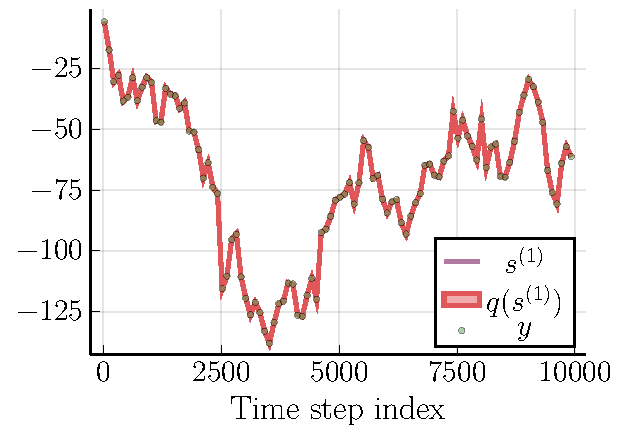
\includegraphics{contents/05-experiments/plots/hgf/04-hierarchical_example_inference_states_2.pdf}
    }
    \caption{Simulated evolution of the layer $s_t^{(1)}$ and its corresponding inferred posterior distribution.}
    \label{fig:sim:hgf_inference_state_1}
  \end{subfigure}
  \hfill
  \begin{subfigure}[t]{0.315\textwidth}
    \centering
    \resizebox{\textwidth}{!}{
        % % Recommended preamble:
% \usetikzlibrary{arrows.meta}
% \usetikzlibrary{backgrounds}
% \usepgfplotslibrary{patchplots}
% \usepgfplotslibrary{fillbetween}
% \pgfplotsset{%
%     layers/standard/.define layer set={%
%         background,axis background,axis grid,axis ticks,axis lines,axis tick labels,pre main,main,axis descriptions,axis foreground%
%     }{
%         grid style={/pgfplots/on layer=axis grid},%
%         tick style={/pgfplots/on layer=axis ticks},%
%         axis line style={/pgfplots/on layer=axis lines},%
%         label style={/pgfplots/on layer=axis descriptions},%
%         legend style={/pgfplots/on layer=axis descriptions},%
%         title style={/pgfplots/on layer=axis descriptions},%
%         colorbar style={/pgfplots/on layer=axis descriptions},%
%         ticklabel style={/pgfplots/on layer=axis tick labels},%
%         axis background@ style={/pgfplots/on layer=axis background},%
%         3d box foreground style={/pgfplots/on layer=axis foreground},%
%     },
% }

\begin{tikzpicture}[/tikz/background rectangle/.style={fill={rgb,1:red,1.0;green,1.0;blue,1.0}, fill opacity={1.0}, draw opacity={1.0}}, show background rectangle]
\begin{axis}[point meta max={nan}, point meta min={nan}, legend cell align={left}, legend columns={1}, title={}, title style={at={{(0.5,1)}}, anchor={south}, font={{\fontsize{18 pt}{23.400000000000002 pt}\selectfont}}, color={rgb,1:red,0.0;green,0.0;blue,0.0}, draw opacity={1.0}, rotate={0.0}, align={center}}, legend style={color={rgb,1:red,0.0;green,0.0;blue,0.0}, draw opacity={1.0}, line width={1}, solid, fill={rgb,1:red,1.0;green,1.0;blue,1.0}, fill opacity={1.0}, text opacity={1.0}, font={{\fontsize{14 pt}{18.2 pt}\selectfont}}, text={rgb,1:red,0.0;green,0.0;blue,0.0}, cells={anchor={center}}, at={(0.98, 0.98)}, anchor={north east}}, axis background/.style={fill={rgb,1:red,1.0;green,1.0;blue,1.0}, opacity={1.0}}, anchor={north west}, xshift={1.0mm}, yshift={-1.0mm}, width={99.6mm}, height={74.2mm}, scaled x ticks={false}, xlabel={Variational iteration index}, x tick style={color={rgb,1:red,0.0;green,0.0;blue,0.0}, opacity={1.0}}, x tick label style={color={rgb,1:red,0.0;green,0.0;blue,0.0}, opacity={1.0}, rotate={0}}, xlabel style={at={(ticklabel cs:0.5)}, anchor=near ticklabel, at={{(ticklabel cs:0.5)}}, anchor={near ticklabel}, font={{\fontsize{16 pt}{20.8 pt}\selectfont}}, color={rgb,1:red,0.0;green,0.0;blue,0.0}, draw opacity={1.0}, rotate={0.0}}, xmajorgrids={true}, xmin={0.8799999999999999}, xmax={5.12}, xticklabels={{$1$,$2$,$3$,$4$,$5$}}, xtick={{1.0,2.0,3.0,4.0,5.0}}, xtick align={inside}, xticklabel style={font={{\fontsize{14 pt}{18.2 pt}\selectfont}}, color={rgb,1:red,0.0;green,0.0;blue,0.0}, draw opacity={1.0}, rotate={0.0}}, x grid style={color={rgb,1:red,0.0;green,0.0;blue,0.0}, draw opacity={0.1}, line width={0.5}, solid}, axis x line*={left}, x axis line style={color={rgb,1:red,0.0;green,0.0;blue,0.0}, draw opacity={1.0}, line width={1}, solid}, scaled y ticks={false}, ylabel={Bethe Free Energy}, y tick style={color={rgb,1:red,0.0;green,0.0;blue,0.0}, opacity={1.0}}, y tick label style={color={rgb,1:red,0.0;green,0.0;blue,0.0}, opacity={1.0}, rotate={0}}, ylabel style={at={(ticklabel cs:0.5)}, anchor=near ticklabel, at={{(ticklabel cs:0.5)}}, anchor={near ticklabel}, font={{\fontsize{16 pt}{20.8 pt}\selectfont}}, color={rgb,1:red,0.0;green,0.0;blue,0.0}, draw opacity={1.0}, rotate={0.0}}, ymajorgrids={true}, ymin={1.3537661894130288}, ymax={1.3588737379406222}, yticklabels={{$1.354$,$1.355$,$1.356$,$1.357$,$1.358$}}, ytick={{1.354,1.355,1.356,1.357,1.358}}, ytick align={inside}, yticklabel style={font={{\fontsize{14 pt}{18.2 pt}\selectfont}}, color={rgb,1:red,0.0;green,0.0;blue,0.0}, draw opacity={1.0}, rotate={0.0}}, y grid style={color={rgb,1:red,0.0;green,0.0;blue,0.0}, draw opacity={0.1}, line width={0.5}, solid}, axis y line*={left}, y axis line style={color={rgb,1:red,0.0;green,0.0;blue,0.0}, draw opacity={1.0}, line width={1}, solid}, colorbar={false}]
    \addplot[color={rgb,1:red,0.0;green,0.6056;blue,0.9787}, name path={febf5715-4f1a-486f-9887-7772927a61c8}, draw opacity={1.0}, line width={1}, solid]
        table[row sep={\\}]
        {
            \\
            1.0  1.3587291846804073  \\
            2.0  1.35401669218457  \\
            3.0  1.353921610870807  \\
            4.0  1.3539111089404197  \\
            5.0  1.353910742673244  \\
        }
        ;
    \addlegendentry {Bethe Free Energy}
\end{axis}
\end{tikzpicture}

        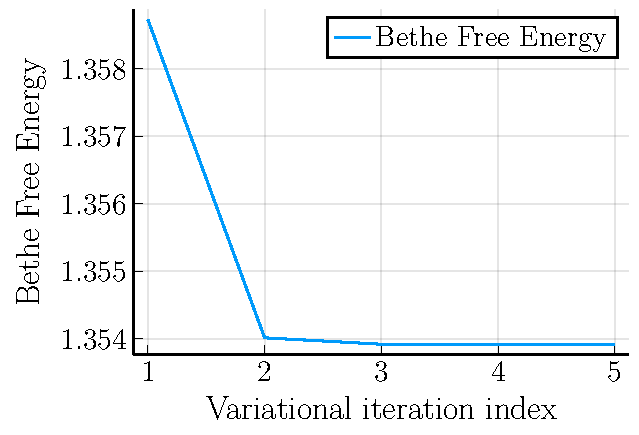
\includegraphics{contents/05-experiments/plots/hgf/04-hierarchical_example_inference_free_energy.pdf}
    }
    \caption{Bethe Free Energy evaluation results.
      The x-axis represents an index of \ac{vmp} iteration.
      The y-axis represents a Bethe Free Energy value at a specific \ac{vmp} iteration.
    }
    \label{fig:sim:hgf_inference_free_energy}
  \end{subfigure}
  \caption{
    Simulated evolution of the 2-layer \ac{hgf} model \eqref{eq:sim:hgf} for $10,000$ synthetically generated 1-dimensional observations with link function $f(s) = exp(\kappa s + \zeta)$, where $\kappa = 1$ and $\zeta = 0$.
    The noise component $\Sigma$ is set to be $10^{-4}$, the noise component $\Omega$ is set to be
    $0.0625$.
    The shaded area shows three standard deviations of the inferred posteriors.
  }
  \label{fig:sim:hgf_inference_states}
\end{figure}

\subsection{Scalability and performance characteristics}

\begin{figure}
  \centering
  \resizebox{\textwidth}{!}{
    % % Recommended preamble:
% \usetikzlibrary{arrows.meta}
% \usetikzlibrary{backgrounds}
% \usepgfplotslibrary{patchplots}
% \usepgfplotslibrary{fillbetween}
% \pgfplotsset{%
%     layers/standard/.define layer set={%
%         background,axis background,axis grid,axis ticks,axis lines,axis tick labels,pre main,main,axis descriptions,axis foreground%
%     }{
%         grid style={/pgfplots/on layer=axis grid},%
%         tick style={/pgfplots/on layer=axis ticks},%
%         axis line style={/pgfplots/on layer=axis lines},%
%         label style={/pgfplots/on layer=axis descriptions},%
%         legend style={/pgfplots/on layer=axis descriptions},%
%         title style={/pgfplots/on layer=axis descriptions},%
%         colorbar style={/pgfplots/on layer=axis descriptions},%
%         ticklabel style={/pgfplots/on layer=axis tick labels},%
%         axis background@ style={/pgfplots/on layer=axis background},%
%         3d box foreground style={/pgfplots/on layer=axis foreground},%
%     },
% }

\begin{tikzpicture}[/tikz/background rectangle/.style={fill={rgb,1:red,1.0;green,1.0;blue,1.0}, fill opacity={1.0}, draw opacity={1.0}}, show background rectangle]
\begin{axis}[point meta max={nan}, point meta min={nan}, legend cell align={left}, legend columns={1}, title={}, title style={at={{(0.5,1)}}, anchor={south}, font={{\fontsize{18 pt}{23.400000000000002 pt}\selectfont}}, color={rgb,1:red,0.0;green,0.0;blue,0.0}, draw opacity={1.0}, rotate={0.0}, align={center}}, legend style={color={rgb,1:red,0.0;green,0.0;blue,0.0}, draw opacity={1.0}, line width={1}, solid, fill={rgb,1:red,1.0;green,1.0;blue,1.0}, fill opacity={1.0}, text opacity={1.0}, font={{\fontsize{14 pt}{18.2 pt}\selectfont}}, text={rgb,1:red,0.0;green,0.0;blue,0.0}, cells={anchor={west}}, at={(0.98, 0.02)}, anchor={south east}}, axis background/.style={fill={rgb,1:red,1.0;green,1.0;blue,1.0}, opacity={1.0}}, anchor={north west}, xshift={1.0mm}, yshift={-1.0mm}, width={226.6mm}, height={86.9mm}, scaled x ticks={false}, xlabel={Number of observation (log-scale)}, x tick style={color={rgb,1:red,0.0;green,0.0;blue,0.0}, opacity={1.0}}, x tick label style={color={rgb,1:red,0.0;green,0.0;blue,0.0}, opacity={1.0}, rotate={0}}, xlabel style={at={(ticklabel cs:0.5)}, anchor=near ticklabel, at={{(ticklabel cs:0.5)}}, anchor={near ticklabel}, font={{\fontsize{16 pt}{20.8 pt}\selectfont}}, color={rgb,1:red,0.0;green,0.0;blue,0.0}, draw opacity={1.0}, rotate={0.0}}, xmode={log}, log basis x={10}, xmajorgrids={true}, xmin={7.585775750291836}, xmax={131825.67385564075}, xticklabels={{$10^1$,$10^2$,$10^3$,$10^4$,$10^5$}}, xtick={{10,100,1000,10000,100000}}, xtick align={inside}, xticklabel style={font={{\fontsize{14 pt}{18.2 pt}\selectfont}}, color={rgb,1:red,0.0;green,0.0;blue,0.0}, draw opacity={1.0}, rotate={0.0}}, x grid style={color={rgb,1:red,0.0;green,0.0;blue,0.0}, draw opacity={0.1}, line width={0.5}, solid}, axis x line*={left}, x axis line style={color={rgb,1:red,0.0;green,0.0;blue,0.0}, draw opacity={1.0}, line width={1}, solid}, scaled y ticks={false}, ylabel={Time (in ms, log-scale)}, y tick style={color={rgb,1:red,0.0;green,0.0;blue,0.0}, opacity={1.0}}, y tick label style={color={rgb,1:red,0.0;green,0.0;blue,0.0}, opacity={1.0}, rotate={0}}, ylabel style={at={(ticklabel cs:0.5)}, anchor=near ticklabel, at={{(ticklabel cs:0.5)}}, anchor={near ticklabel}, font={{\fontsize{16 pt}{20.8 pt}\selectfont}}, color={rgb,1:red,0.0;green,0.0;blue,0.0}, draw opacity={1.0}, rotate={0.0}}, ymode={log}, log basis y={10}, ymajorgrids={true}, ymin={0.1}, ymax={1.0e6}, yticklabels={{$10^{-1}$,$10^{0}$,$10^{1}$,$10^{2}$,$10^{3}$,$10^{4}$,$10^5$,$10^6$}}, ytick={{0.1,1.0,10.0,100.0,1000.0,10000.0,100000.0,1.0e6}}, ytick align={inside}, yticklabel style={font={{\fontsize{14 pt}{18.2 pt}\selectfont}}, color={rgb,1:red,0.0;green,0.0;blue,0.0}, draw opacity={1.0}, rotate={0.0}}, y grid style={color={rgb,1:red,0.0;green,0.0;blue,0.0}, draw opacity={0.1}, line width={0.5}, solid}, axis y line*={left}, y axis line style={color={rgb,1:red,0.0;green,0.0;blue,0.0}, draw opacity={1.0}, line width={1}, solid}, colorbar={false}]
    \addplot[color={rgb,1:red,0.0;green,0.6056;blue,0.9787}, name path={b15436e0-7789-44d4-adba-9fd4d8234e94}, draw opacity={1.0}, line width={1}, solid, mark={triangle*}, mark size={3.0 pt}, mark repeat={1}, mark options={color={rgb,1:red,0.0;green,0.0;blue,0.0}, draw opacity={1.0}, fill={rgb,1:red,0.0;green,0.6056;blue,0.9787}, fill opacity={1.0}, line width={0.75}, rotate={0}, solid}]
        table[row sep={\\}]
        {
            \\
            10.0  0.4315  \\
            20.0  0.7331  \\
            30.0  1.0663  \\
            100.0  3.1955  \\
            300.0  9.3212  \\
            500.0  15.4309  \\
            700.0  21.7392  \\
            1000.0  30.9804  \\
            3000.0  92.092  \\
            5000.0  155.2424  \\
            7000.0  216.4502  \\
            10000.0  306.9206  \\
            30000.0  979.1397  \\
            50000.0  1562.5644  \\
            70000.0  2215.5032  \\
            100000.0  3165.3835  \\
        }
        ;
    \addlegendentry {Reactive MP}
    \addplot[color={rgb,1:red,0.8889;green,0.4356;blue,0.2781}, name path={9f987ce9-b428-449b-ab6f-d128750f590d}, draw opacity={1.0}, line width={1}, dashed, mark={triangle*}, mark size={3.0 pt}, mark repeat={1}, mark options={color={rgb,1:red,0.0;green,0.0;blue,0.0}, draw opacity={1.0}, fill={rgb,1:red,0.8889;green,0.4356;blue,0.2781}, fill opacity={1.0}, line width={0.75}, rotate={180}, solid}]
        table[row sep={\\}]
        {
            \\
            10.0  6.7619  \\
            20.0  13.5798  \\
            30.0  20.4546  \\
            100.0  68.2079  \\
            300.0  206.7111  \\
        }
        ;
    \addlegendentry {Scheduled MP (inference)}
    \addplot[color={rgb,1:red,0.2422;green,0.6433;blue,0.3044}, name path={c238d3f5-cd32-4311-8dcb-ec179cc65982}, draw opacity={1.0}, line width={1}, dashed, mark={triangle*}, mark size={3.0 pt}, mark repeat={1}, mark options={color={rgb,1:red,0.0;green,0.0;blue,0.0}, draw opacity={1.0}, fill={rgb,1:red,0.2422;green,0.6433;blue,0.3044}, fill opacity={1.0}, line width={0.75}, rotate={270}, solid}]
        table[row sep={\\}]
        {
            \\
            10.0  252.56  \\
            20.0  257.965  \\
            30.0  257.8601  \\
            100.0  257.6473  \\
            300.0  255.883  \\
        }
        ;
    \addlegendentry {Scheduled MP (compilation)}
    \addplot[color={rgb,1:red,0.7644;green,0.4441;blue,0.8243}, name path={2150c3b6-9adb-4c15-aadd-118c7691217b}, draw opacity={1.0}, line width={1}, dotted, mark={triangle*}, mark size={3.0 pt}, mark repeat={1}, mark options={color={rgb,1:red,0.0;green,0.0;blue,0.0}, draw opacity={1.0}, fill={rgb,1:red,0.7644;green,0.4441;blue,0.8243}, fill opacity={1.0}, line width={0.75}, rotate={90}, solid}]
        table[row sep={\\}]
        {
            \\
            10.0  3866.7066  \\
            20.0  8099.2013  \\
            30.0  12282.4029  \\
            100.0  41746.4358  \\
            300.0  120336.0759  \\
        }
        ;
    \addlegendentry {NUTS (100)}
    \addplot[color={rgb,1:red,0.6755;green,0.5557;blue,0.0942}, name path={08d41fab-29aa-42f9-a576-5f85198b2541}, draw opacity={1.0}, line width={1}, dotted, mark={diamond*}, mark size={3.0 pt}, mark repeat={1}, mark options={color={rgb,1:red,0.0;green,0.0;blue,0.0}, draw opacity={1.0}, fill={rgb,1:red,0.6755;green,0.5557;blue,0.0942}, fill opacity={1.0}, line width={0.75}, rotate={0}, solid}]
        table[row sep={\\}]
        {
            \\
            10.0  9051.1129  \\
            20.0  18286.9567  \\
            30.0  27829.6717  \\
            100.0  89140.8722  \\
            300.0  264435.7674  \\
        }
        ;
    \addlegendentry {NUTS (200)}
\end{axis}
\end{tikzpicture}

    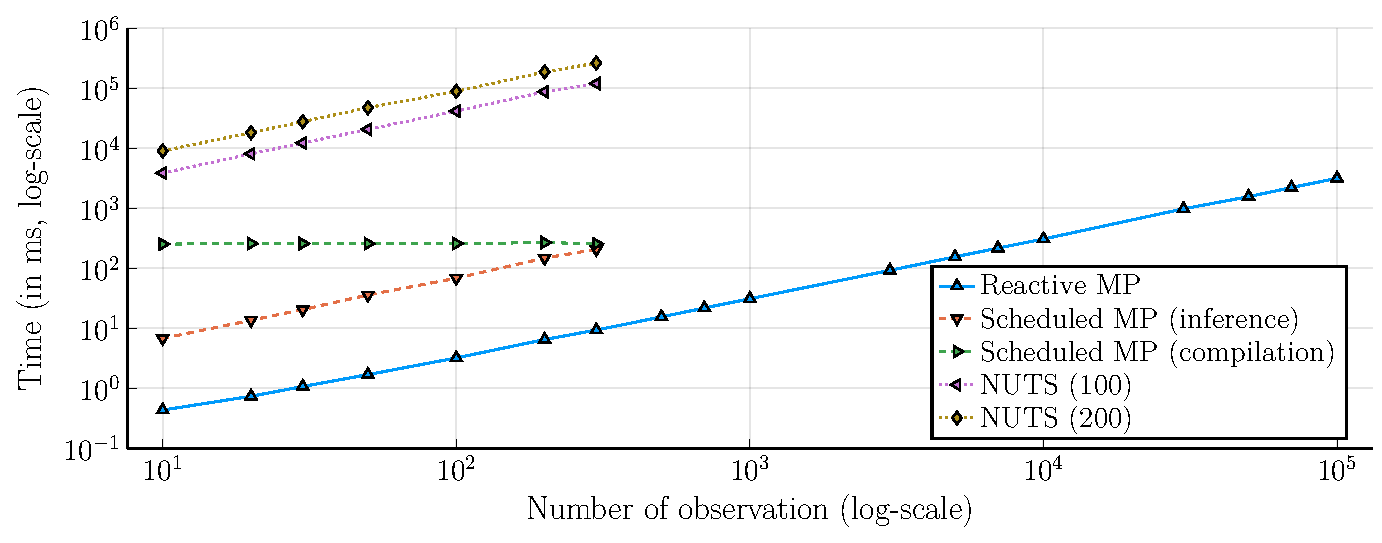
\includegraphics{contents/05-experiments/plots/hgf/04-benchmark_comparison.pdf}
  }
  \caption{A comparison of the runtime duration in milliseconds for automated Bayesian inference in a 2-layer \ac{hgf}~\eqref{eq:sim:hgf} using different methods: reactive message passing (RxInfer), scheduled message passing (ForneyLab), and \ac{nuts} (Turing).
    The values in the figure represent the minimum duration across multiple runs.
    The RxInfer timings include the graph creation time.
    The ForneyLab pipeline involves model compilation, followed by actual inference execution.
    Turing uses \ac{nuts} sampling with 100 and 200 samples, respectively.
    We present benchmark results for more than $300$ observations only for the RxInfer framework.
  }
  \label{fig:sim:hgf_performance_comparison}
\end{figure}

\begin{table}[t]
  \centering
  \begin{tabular}{ |l||r|r|r|r|r|r| }
    \hline
                  & \multicolumn{6}{|c|}{Number of observations}                                                                            \\
    \hline
                  & \multicolumn{3}{|c|}{$s^{(2)}_t$ layer}      & \multicolumn{3}{|c|}{$s^{(1)_t}$ layer}                                  \\
    \hline
                  & 50                                           & 100                                     & 200  & 50    & 100    & 200    \\
    \hline
    VMP (5 iters) & 0.30                                         & 0.18                                    & 0.12 & 0.16  & 0.15   & 0.15   \\
    \hline
    NUTS (100)    & 0.34                                         & 0.27                                    & 0.26 & 65.86 & 140.96 & 364.40 \\
    NUTS (200)    & 0.18                                         & 0.30                                    & 0.14 & 69.01 & 147.88 & 365.02 \\
    \hline
  \end{tabular}
  \caption{Comparison of posterior results accuracy in terms of metric \eqref{eq:sim:average_mse} in the \ac{hgf}~\eqref{eq:sim:hgf} across different methods: message passing (RxInfer and ForneyLab) and \ac{nuts} (Turing).
    Lower values indicate better performance.
    RxInfer and ForneyLab perform online learning with \ac{vmp} on a single time step of the
    corresponding graph.
    The number of \ac{vmp} iterations is set to 5.
    Turing.jl runs two benchmarks with 100 and 200 number of samples respectively.
  }
  \label{table:sim:hgf_accuracy_comparison}
\end{table}

\begin{figure}
  \centering
  \begin{subfigure}[t]{\textwidth}
    \centering
    \resizebox{\textwidth}{!}{
        % % Recommended preamble:
% \usetikzlibrary{arrows.meta}
% \usetikzlibrary{backgrounds}
% \usepgfplotslibrary{patchplots}
% \usepgfplotslibrary{fillbetween}
% \pgfplotsset{%
%     layers/standard/.define layer set={%
%         background,axis background,axis grid,axis ticks,axis lines,axis tick labels,pre main,main,axis descriptions,axis foreground%
%     }{
%         grid style={/pgfplots/on layer=axis grid},%
%         tick style={/pgfplots/on layer=axis ticks},%
%         axis line style={/pgfplots/on layer=axis lines},%
%         label style={/pgfplots/on layer=axis descriptions},%
%         legend style={/pgfplots/on layer=axis descriptions},%
%         title style={/pgfplots/on layer=axis descriptions},%
%         colorbar style={/pgfplots/on layer=axis descriptions},%
%         ticklabel style={/pgfplots/on layer=axis tick labels},%
%         axis background@ style={/pgfplots/on layer=axis background},%
%         3d box foreground style={/pgfplots/on layer=axis foreground},%
%     },
% }

\begin{tikzpicture}[/tikz/background rectangle/.style={fill={rgb,1:red,1.0;green,1.0;blue,1.0}, fill opacity={1.0}, draw opacity={1.0}}, show background rectangle]
\begin{axis}[point meta max={nan}, point meta min={nan}, legend cell align={left}, legend columns={2}, title={}, title style={at={{(0.5,1)}}, anchor={south}, font={{\fontsize{18 pt}{23.400000000000002 pt}\selectfont}}, color={rgb,1:red,0.0;green,0.0;blue,0.0}, draw opacity={1.0}, rotate={0.0}, align={center}}, legend style={color={rgb,1:red,0.0;green,0.0;blue,0.0}, draw opacity={1.0}, line width={1}, solid, fill={rgb,1:red,1.0;green,1.0;blue,1.0}, fill opacity={1.0}, text opacity={1.0}, font={{\fontsize{14 pt}{18.2 pt}\selectfont}}, text={rgb,1:red,0.0;green,0.0;blue,0.0}, cells={anchor={west}}, at={(0.5, 1.02)}, anchor={south}}, axis background/.style={fill={rgb,1:red,1.0;green,1.0;blue,1.0}, opacity={1.0}}, anchor={north west}, xshift={1.0mm}, yshift={-1.0mm}, width={201.2mm}, height={74.2mm}, scaled x ticks={false}, xlabel={Number of observations in dataset (log10-scale)}, x tick style={color={rgb,1:red,0.0;green,0.0;blue,0.0}, opacity={1.0}}, x tick label style={color={rgb,1:red,0.0;green,0.0;blue,0.0}, opacity={1.0}, rotate={0}}, xlabel style={at={(ticklabel cs:0.5)}, anchor=near ticklabel, at={{(ticklabel cs:0.5)}}, anchor={near ticklabel}, font={{\fontsize{16 pt}{20.8 pt}\selectfont}}, color={rgb,1:red,0.0;green,0.0;blue,0.0}, draw opacity={1.0}, rotate={0.0}}, xmode={log}, log basis x={10}, xmajorgrids={true}, xmin={7.585775750291836}, xmax={131825.67385564075}, xticklabels={{$10^1$,$10^2$,$10^3$,$10^4$,$10^5$}}, xtick={{10,100,1000,10000,100000}}, xtick align={inside}, xticklabel style={font={{\fontsize{14 pt}{18.2 pt}\selectfont}}, color={rgb,1:red,0.0;green,0.0;blue,0.0}, draw opacity={1.0}, rotate={0.0}}, x grid style={color={rgb,1:red,0.0;green,0.0;blue,0.0}, draw opacity={0.1}, line width={0.5}, solid}, axis x line*={left}, x axis line style={color={rgb,1:red,0.0;green,0.0;blue,0.0}, draw opacity={1.0}, line width={1}, solid}, scaled y ticks={false}, ylabel={Time (in ms, log10-scale)}, y tick style={color={rgb,1:red,0.0;green,0.0;blue,0.0}, opacity={1.0}}, y tick label style={color={rgb,1:red,0.0;green,0.0;blue,0.0}, opacity={1.0}, rotate={0}}, ylabel style={at={(ticklabel cs:0.5)}, anchor=near ticklabel, at={{(ticklabel cs:0.5)}}, anchor={near ticklabel}, font={{\fontsize{16 pt}{20.8 pt}\selectfont}}, color={rgb,1:red,0.0;green,0.0;blue,0.0}, draw opacity={1.0}, rotate={0.0}}, ymode={log}, log basis y={10}, ymajorgrids={true}, ymin={0.1}, ymax={100000.0}, yticklabels={{$10^{-1}$,$10^{0}$,$10^{1}$,$10^{2}$,$10^{3}$,$10^{4}$,$10^{5}$}}, ytick={{0.1,1.0,10.0,100.0,1000.0,10000.0,100000.0}}, ytick align={inside}, yticklabel style={font={{\fontsize{14 pt}{18.2 pt}\selectfont}}, color={rgb,1:red,0.0;green,0.0;blue,0.0}, draw opacity={1.0}, rotate={0.0}}, y grid style={color={rgb,1:red,0.0;green,0.0;blue,0.0}, draw opacity={0.1}, line width={0.5}, solid}, axis y line*={left}, y axis line style={color={rgb,1:red,0.0;green,0.0;blue,0.0}, draw opacity={1.0}, line width={1}, solid}, colorbar={false}]
    \addplot[color={rgb,1:red,0.3059;green,0.4745;blue,0.6549}, name path={d581c56f-aaf1-4633-a50f-ab6d23cf33f9}, draw opacity={1.0}, line width={1}, solid, mark={diamond*}, mark size={3.0 pt}, mark repeat={1}, mark options={color={rgb,1:red,0.0;green,0.0;blue,0.0}, draw opacity={1.0}, fill={rgb,1:red,0.3059;green,0.4745;blue,0.6549}, fill opacity={1.0}, line width={0.75}, rotate={0}, solid}]
        table[row sep={\\}]
        {
            \\
            10.0  0.4315  \\
            20.0  0.7331  \\
            30.0  1.0663  \\
            50.0  1.6845  \\
            100.0  3.1955  \\
            200.0  6.4795  \\
            300.0  9.3212  \\
            500.0  15.4309  \\
            700.0  21.7392  \\
            1000.0  30.9804  \\
            3000.0  92.092  \\
            5000.0  155.2424  \\
            7000.0  216.4502  \\
            10000.0  306.9206  \\
            30000.0  979.1397  \\
            50000.0  1562.5644  \\
            70000.0  2215.5032  \\
            100000.0  3165.3835  \\
        }
        ;
    \addlegendentry {3 iterations}
    \addplot[color={rgb,1:red,0.949;green,0.5569;blue,0.1686}, name path={74fe8840-82b9-4868-ad3a-b3cccd6e7e94}, draw opacity={1.0}, line width={1}, dashed, mark={*}, mark size={3.0 pt}, mark repeat={1}, mark options={color={rgb,1:red,0.0;green,0.0;blue,0.0}, draw opacity={1.0}, fill={rgb,1:red,0.949;green,0.5569;blue,0.1686}, fill opacity={1.0}, line width={0.75}, rotate={0}, solid}]
        table[row sep={\\}]
        {
            \\
            10.0  0.6456  \\
            20.0  1.1567  \\
            30.0  1.6744  \\
            50.0  2.7448  \\
            100.0  5.1953  \\
            200.0  10.6134  \\
            300.0  15.4119  \\
            500.0  25.5958  \\
            700.0  35.7002  \\
            1000.0  51.1289  \\
            3000.0  152.9888  \\
            5000.0  255.4111  \\
            7000.0  366.5118  \\
            10000.0  512.6566  \\
            30000.0  1546.797  \\
            50000.0  2662.1589  \\
            70000.0  3661.5947  \\
            100000.0  5162.338  \\
        }
        ;
    \addlegendentry {5 iterations}
    \addplot[color={rgb,1:red,0.8824;green,0.3412;blue,0.349}, name path={66f78ad3-ebb7-4c6d-b85f-b06816b2d7dd}, draw opacity={1.0}, line width={1}, dotted, mark={square*}, mark size={3.0 pt}, mark repeat={1}, mark options={color={rgb,1:red,0.0;green,0.0;blue,0.0}, draw opacity={1.0}, fill={rgb,1:red,0.8824;green,0.3412;blue,0.349}, fill opacity={1.0}, line width={0.75}, rotate={0}, solid}]
        table[row sep={\\}]
        {
            \\
            10.0  1.1486  \\
            20.0  2.1796  \\
            30.0  3.1385  \\
            50.0  5.3404  \\
            100.0  10.2956  \\
            200.0  20.9034  \\
            300.0  30.7604  \\
            500.0  51.0307  \\
            700.0  71.0889  \\
            1000.0  101.6726  \\
            3000.0  306.3463  \\
            5000.0  507.9857  \\
            7000.0  730.3044  \\
            10000.0  1023.7101  \\
            30000.0  3135.6569  \\
            50000.0  5125.1793  \\
            70000.0  7378.6533  \\
            100000.0  10502.3322  \\
        }
        ;
    \addlegendentry {10 iterations}
    \addplot[color={rgb,1:red,0.4627;green,0.7176;blue,0.698}, name path={089c873d-8bf7-40d5-854e-0b2b96b48420}, draw opacity={1.0}, line width={1}, dashdotted, mark={triangle*}, mark size={3.0 pt}, mark repeat={1}, mark options={color={rgb,1:red,0.0;green,0.0;blue,0.0}, draw opacity={1.0}, fill={rgb,1:red,0.4627;green,0.7176;blue,0.698}, fill opacity={1.0}, line width={0.75}, rotate={0}, solid}]
        table[row sep={\\}]
        {
            \\
            10.0  2.1807  \\
            20.0  4.183  \\
            30.0  6.1758  \\
            50.0  10.5072  \\
            100.0  20.5674  \\
            200.0  42.5915  \\
            300.0  60.7581  \\
            500.0  101.6792  \\
            700.0  141.984  \\
            1000.0  205.3108  \\
            3000.0  611.7559  \\
            5000.0  1021.3451  \\
            7000.0  1428.5972  \\
            10000.0  2078.2337  \\
            30000.0  6293.4465  \\
            50000.0  10292.5744  \\
            70000.0  14479.5076  \\
            100000.0  20609.9497  \\
        }
        ;
    \addlegendentry {20 iterations}
\end{axis}
\end{tikzpicture}

        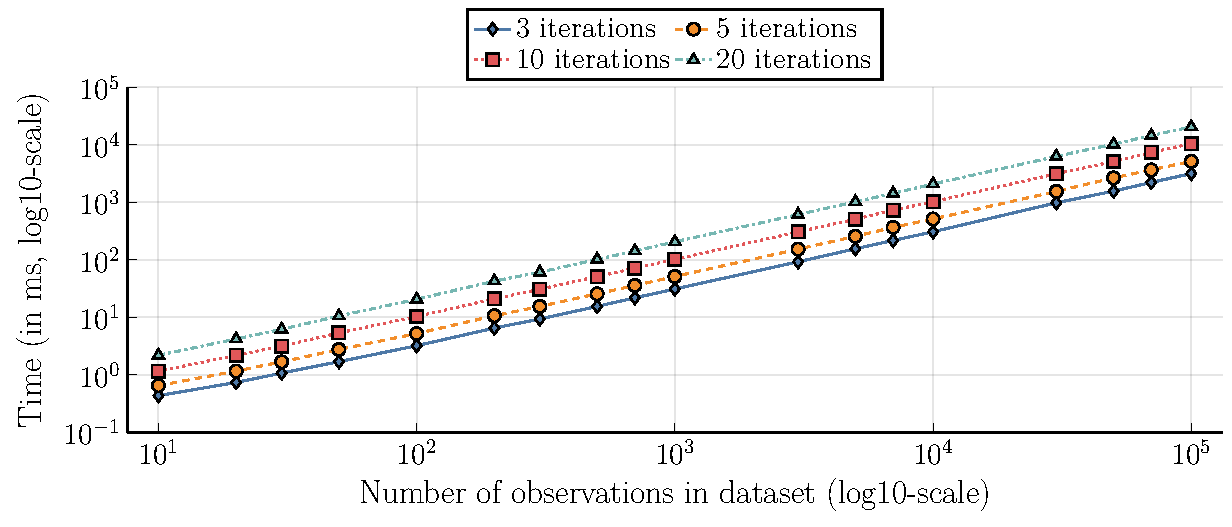
\includegraphics{contents/05-experiments/plots/hgf/04-rxinfer_hgf_scalability_size.pdf}
    }
    \caption{
      Scalability benchmark for different number of performed \ac{vmp} iterations with respect to number of observations in dataset.
    }
    \label{fig:sim:hgf_scalability_size}
  \end{subfigure}
  \hfill
  \begin{subfigure}[t]{\textwidth}
    \centering
    \resizebox{\textwidth}{!}{
        % % Recommended preamble:
% \usetikzlibrary{arrows.meta}
% \usetikzlibrary{backgrounds}
% \usepgfplotslibrary{patchplots}
% \usepgfplotslibrary{fillbetween}
% \pgfplotsset{%
%     layers/standard/.define layer set={%
%         background,axis background,axis grid,axis ticks,axis lines,axis tick labels,pre main,main,axis descriptions,axis foreground%
%     }{
%         grid style={/pgfplots/on layer=axis grid},%
%         tick style={/pgfplots/on layer=axis ticks},%
%         axis line style={/pgfplots/on layer=axis lines},%
%         label style={/pgfplots/on layer=axis descriptions},%
%         legend style={/pgfplots/on layer=axis descriptions},%
%         title style={/pgfplots/on layer=axis descriptions},%
%         colorbar style={/pgfplots/on layer=axis descriptions},%
%         ticklabel style={/pgfplots/on layer=axis tick labels},%
%         axis background@ style={/pgfplots/on layer=axis background},%
%         3d box foreground style={/pgfplots/on layer=axis foreground},%
%     },
% }

\begin{tikzpicture}[/tikz/background rectangle/.style={fill={rgb,1:red,1.0;green,1.0;blue,1.0}, fill opacity={1.0}, draw opacity={1.0}}, show background rectangle]
\begin{axis}[point meta max={nan}, point meta min={nan}, legend cell align={left}, legend columns={2}, title={}, title style={at={{(0.5,1)}}, anchor={south}, font={{\fontsize{18 pt}{23.400000000000002 pt}\selectfont}}, color={rgb,1:red,0.0;green,0.0;blue,0.0}, draw opacity={1.0}, rotate={0.0}, align={center}}, legend style={color={rgb,1:red,0.0;green,0.0;blue,0.0}, draw opacity={1.0}, line width={1}, solid, fill={rgb,1:red,1.0;green,1.0;blue,1.0}, fill opacity={1.0}, text opacity={1.0}, font={{\fontsize{14 pt}{18.2 pt}\selectfont}}, text={rgb,1:red,0.0;green,0.0;blue,0.0}, cells={anchor={west}}, at={(0.5, 1.02)}, anchor={south}}, axis background/.style={fill={rgb,1:red,1.0;green,1.0;blue,1.0}, opacity={1.0}}, anchor={north west}, xshift={1.0mm}, yshift={-1.0mm}, width={201.2mm}, height={74.2mm}, scaled x ticks={false}, xlabel={Number of iterations}, x tick style={color={rgb,1:red,0.0;green,0.0;blue,0.0}, opacity={1.0}}, x tick label style={color={rgb,1:red,0.0;green,0.0;blue,0.0}, opacity={1.0}, rotate={0}}, xlabel style={at={(ticklabel cs:0.5)}, anchor=near ticklabel, at={{(ticklabel cs:0.5)}}, anchor={near ticklabel}, font={{\fontsize{16 pt}{20.8 pt}\selectfont}}, color={rgb,1:red,0.0;green,0.0;blue,0.0}, draw opacity={1.0}, rotate={0.0}}, xmajorgrids={true}, xmin={2.49}, xmax={20.509999999999998}, xticklabels={{3,5,10,20}}, xtick={{3,5,10,20}}, xtick align={inside}, xticklabel style={font={{\fontsize{14 pt}{18.2 pt}\selectfont}}, color={rgb,1:red,0.0;green,0.0;blue,0.0}, draw opacity={1.0}, rotate={0.0}}, x grid style={color={rgb,1:red,0.0;green,0.0;blue,0.0}, draw opacity={0.1}, line width={0.5}, solid}, axis x line*={left}, x axis line style={color={rgb,1:red,0.0;green,0.0;blue,0.0}, draw opacity={1.0}, line width={1}, solid}, scaled y ticks={false}, ylabel={Time (in ms, log10-scale)}, y tick style={color={rgb,1:red,0.0;green,0.0;blue,0.0}, opacity={1.0}}, y tick label style={color={rgb,1:red,0.0;green,0.0;blue,0.0}, opacity={1.0}, rotate={0}}, ylabel style={at={(ticklabel cs:0.5)}, anchor=near ticklabel, at={{(ticklabel cs:0.5)}}, anchor={near ticklabel}, font={{\fontsize{16 pt}{20.8 pt}\selectfont}}, color={rgb,1:red,0.0;green,0.0;blue,0.0}, draw opacity={1.0}, rotate={0.0}}, ymode={log}, log basis y={10}, ymajorgrids={true}, ymin={0.1}, ymax={100000.0}, yticklabels={{$10^{-1}$,$10^{0}$,$10^{1}$,$10^{2}$,$10^{3}$,$10^{4}$,$10^{5}$}}, ytick={{0.1,1.0,10.0,100.0,1000.0,10000.0,100000.0}}, ytick align={inside}, yticklabel style={font={{\fontsize{14 pt}{18.2 pt}\selectfont}}, color={rgb,1:red,0.0;green,0.0;blue,0.0}, draw opacity={1.0}, rotate={0.0}}, y grid style={color={rgb,1:red,0.0;green,0.0;blue,0.0}, draw opacity={0.1}, line width={0.5}, solid}, axis y line*={left}, y axis line style={color={rgb,1:red,0.0;green,0.0;blue,0.0}, draw opacity={1.0}, line width={1}, solid}, colorbar={false}]
    \addplot[color={rgb,1:red,0.3059;green,0.4745;blue,0.6549}, name path={7686c7b2-1869-4449-bf45-8f7efc6fec72}, draw opacity={1.0}, line width={1}, solid, mark={triangle*}, mark size={3.0 pt}, mark repeat={1}, mark options={color={rgb,1:red,0.0;green,0.0;blue,0.0}, draw opacity={1.0}, fill={rgb,1:red,0.3059;green,0.4745;blue,0.6549}, fill opacity={1.0}, line width={0.75}, rotate={0}, solid}]
        table[row sep={\\}]
        {
            \\
            3.0  0.4315  \\
            5.0  0.6456  \\
            10.0  1.1486  \\
            20.0  2.1807  \\
        }
        ;
    \addlegendentry {10 observations}
    \addplot[color={rgb,1:red,0.949;green,0.5569;blue,0.1686}, name path={509ac5b6-83f7-4989-ac40-3ef533f522a7}, draw opacity={1.0}, line width={1}, dashed, mark={triangle*}, mark size={3.0 pt}, mark repeat={1}, mark options={color={rgb,1:red,0.0;green,0.0;blue,0.0}, draw opacity={1.0}, fill={rgb,1:red,0.949;green,0.5569;blue,0.1686}, fill opacity={1.0}, line width={0.75}, rotate={180}, solid}]
        table[row sep={\\}]
        {
            \\
            3.0  30.9804  \\
            5.0  51.1289  \\
            10.0  101.6726  \\
            20.0  205.3108  \\
        }
        ;
    \addlegendentry {1000 observations}
    \addplot[color={rgb,1:red,0.8824;green,0.3412;blue,0.349}, name path={ed9cc609-e972-43ff-9fed-517cace576f3}, draw opacity={1.0}, line width={1}, dotted, mark={triangle*}, mark size={3.0 pt}, mark repeat={1}, mark options={color={rgb,1:red,0.0;green,0.0;blue,0.0}, draw opacity={1.0}, fill={rgb,1:red,0.8824;green,0.3412;blue,0.349}, fill opacity={1.0}, line width={0.75}, rotate={270}, solid}]
        table[row sep={\\}]
        {
            \\
            3.0  306.9206  \\
            5.0  512.6566  \\
            10.0  1023.7101  \\
            20.0  2078.2337  \\
        }
        ;
    \addlegendentry {10000 observations}
    \addplot[color={rgb,1:red,0.4627;green,0.7176;blue,0.698}, name path={c56a334d-6c42-40f8-9491-b35a506ac7f6}, draw opacity={1.0}, line width={1}, dashdotted, mark={triangle*}, mark size={3.0 pt}, mark repeat={1}, mark options={color={rgb,1:red,0.0;green,0.0;blue,0.0}, draw opacity={1.0}, fill={rgb,1:red,0.4627;green,0.7176;blue,0.698}, fill opacity={1.0}, line width={0.75}, rotate={90}, solid}]
        table[row sep={\\}]
        {
            \\
            3.0  3165.3835  \\
            5.0  5162.338  \\
            10.0  10502.3322  \\
            20.0  20609.9497  \\
        }
        ;
    \addlegendentry {100000 observations}
\end{axis}
\end{tikzpicture}

        \includegraphics{contents/05-experiments/plots/hgf/04-rxinfer_hgf_scalability_nits.pdf}
    }
    \caption{Scalability benchmark for different number of observations with respect to number of performed \ac{vmp} iterations.
    }
    \label{fig:sim:hgf_scalability_nits}
  \end{subfigure}
  \caption{    The benchmark for online Bayesian inference for a 2-layer \ac{hgf} system~\eqref{eq:sim:hgf} for RxInfer framework.
    The results demonstrate great scalability of RxInfer framework for different number of
    observations in dataset and for different number of performed \ac{vmp} iterations.
    The values in the table show the minimum possible duration across multiple runs.
    The timings include graph creation time.
  }
  \label{fig:sim:hgf_scalability}
\end{figure}

The main benchmark results are presented in Figure~\ref{fig:sim:hgf_performance_comparison},
and the comparison of the inference accuracy is shown in Table~\ref{table:sim:hgf_accuracy_comparison}.
We demonstrate the performance of the RxInfer framework based on the number of observations
and the number of \ac{vmp} iterations for this particular model in
Figure~\ref{fig:sim:hgf_scalability}.
As in the previous example, we observe that the RxInfer framework scales linearly with both
the number of observations and the number of \ac{vmp} iterations performed (\hyperlink{experiments:scalability}{\emph{Scalability}}).

In this specific example, the inference task in RxInfer for the $10^5$ measurements takes
approximately $3$ seconds, which accounts for $30$ microseconds per measurement.
This efficiency allows the deployment of such models in volatile environments, enabling
real-time continual inference (\hyperlink{experiments:efficiency}{\emph{Run-time efficiency and speed}}).

Unlike the previous examples, where we performed inference on a full graph, the ForneyLab
compilation time no longer depends on the number of observations.
The compilation of the fixed global schedule becomes more acceptable because we always build a single time step of a graph and reuse it during online learning.
Both RxInfer and ForneyLab show the same scalability and posterior accuracy results since they
use the same method for posterior approximation.
However, RxInfer is faster in \ac{vmp} inference execution in absolute timing due to the
architecture proposed in Section~\ref{chapter-03:section:reactive-continual-inference}.
In this architecture, computer resources are used more efficiently as there is no need to
recreate the graph for each new observation of a one-time segment.

In this model, \ac{nuts} algorithm, while being slower in absolute execution time, shows
significantly less accurate results in terms of the metric \eqref{eq:sim:average_mse}, and the
estimated posterior distributions for the first layer start to diverge from their real values  (\hyperlink{experiments:accuracy}{\emph{Posterior accuracy}}).
This outcome may occur because we are restricted to using only one measurement at a time and
performing online (filtering) learning, for which the \ac{nuts} algorithm has not been specifically
designed.
\ac{nuts} typically operates on batches of data, making it difficult to handle streaming data in
real-time scenarios where new observations come one at a time.
Due to these limitations, \ac{nuts} is generally not recommended for real-time dynamical nonstationary
systems, especially when dealing with streaming data or when fast and frequent updates to the
posterior distribution are required.

